\chapter{Basics}
\label{ch:basics}
\section{Einstellungen}
\label{sec:einstellungen}
Über das Personensymbol (\autoref{subsec:Personensymbol}) gelangt man zu den Einstellungen\index{Einstellungen} indem im Dropdown-Menü der entsprechende Reiter ausgewählt wird. In den Einstellungen kann zwischen unterschiedlichen Reitern gewählt werden:
\begin{description}
   \item[Mein Profil:]\index{Mein Profil}
	\item[]
Hier können persönliche Informationen ergänzt werden, die auf der Seite \enquote{meinLebenslauf} dargestellt werden. Im Auswahlmenü \enquote{Profil einsehbar für} wird eingestellt, wer diese Informationen einsehen kann (privat, Freunde, öffentlich). Hier kann auch der Link für die OpenUrl (\autoref{subsec:OpenURL}) hinterlegt werden. \index{OpenURL}
   \item[Einstellungen:] 
   \begin{itemize}
      \item[] % schönerer Umbruch
      \item Anzeige der \tag-Auswahl ändern: Liste oder Wolke
      \item Anzeige der \tag-Reihenfolge ändern: Alphabet oder Häufigkeit
      \item \tag-Tipps: Funktion ist nicht mehr vorhanden
      \item \tag-Auswahl: Top X oder mind. Häufigkeit. Bei TOP X werden nur die X häufigsten \tags angezeigt, bei min. Häufigkeit werden nur die \tags angezeigt die X-Mal vorkommen.
      \item Schrankenwert: Einstellung von X
      \item Einträge pro Seite: Kann bis 10000 hoch gesetzt werden, um im persönlichen Konto die Einträge sortieren zu können. Das Laden dieser Einträge dauert allerdings sehr lange. Empfehlung: Die Sortierung kann über zwei andere Wege gelöst werden \todo{Sortierung referenzieren und an anderer Stelle beschreiben}
      \item \enquote{Bevorzugte Exportformate}: Auswahl von Zitationsstilen, die beim Export als erstes angezeigt werden sollen.
      \item Erscheinungsbild: erweitert oder einfach. Beim einfachen werden einige Funktionen, die nicht unbedingt benötigt werden nicht angezeigt: zum Beispiel werden unter \enquote{mein PUMA} mehr Auswahlfelder angeboten.
      \item Sprachauswahl: deutsch, englisch oder russisch
      \item API-Schlüssel\index{API-Schlüssel}: wird benötigt, um von externen Programmen auf PUMA zuzugreifen. Zum Beispiel für die Einbindung der Literaturliste in OpenCMS. Alternativer Weg über OAUTH \todo[inline]{Referenz setzen und an anderer Stelle beschreiben}
      \item Klick-Aufzeichnungen erlauben: Klicks auf externe Links werden aufgezeichnet, um wissenschaftlich Auswertungen vornehmen zu können ~\autoref{ch:pumaForschungsprojekt}.
      \item Bestätigung vor Löschen: Wenn ein Eintrag gelöscht wird, kann hier ein eingestellt werden, ob noch einmal vor dem löschen nachgefragt werden soll.
      \item PUMA-Konto löschen: hier kann das gesamte Profil gelöscht werden. Aus Sicherheitsgründen kann der Name eines einmal gelöschtes Kontos nicht wieder vergeben werden.
			\end{itemize}
   \item[JabRef Layout-Datei:]\index{JabRef! Layout-Datei} 
	In diesem Reiter können JabRef-Layout-Dateien hochgeladen werden, um Publikationslisten nach eigenen Wünschen darzustellen. Dazu eine einzelne oder die in drei Teile vorhandene Layout-Datei hochladen, und abschicken. Das Layout kann dann unter dem PUMA-Link im Text geöffnet werden. %Dies ist eine Alternative zur \href{http://citationstyles.org/}{Citation Style Language}. PUMA bietet bereits viele dieser Exportmöglichkeiten (~\autoref{ch:exportImport}) an.\footnote{Unter \url{https://github.com/JabRef/layouts.jabref.org} werden weitere Stile angeboten.} Wenn ein Stil für einen erweiterten Personenkreis benötigt wird, kann dieser auf Anfrage in den allgemeinen Export aufgenommen werden.
\begin{tip} Die Jabref-Layout Dateien werden von PUMA nicht mehr weiter entwickelt. Als Alternative wird die die \href{http://citationstyles.org/}{Citation Style Language} angeboten.
\end{tip}
\todo{verweis einfügen und Abscnhitt über csl schreiben}
\item[Lebenslauf\index{Lebenslauf}]
Daten aus dem persönlichen Profil werden anderen Nutzern (Personenkreis je nach Einstellung in \enquote{meinProfil}) in dem hier eingestellten Layout dargestellt. Es kann zwischen unterschiedlichen Layouts ausgewählt werden oder ein eigenes mit Hilfe der MediaWiki-Syntax\footnote{\url{https://en.wikipedia.org/wiki/Help:Wiki_markup}}erstellt werden (~\autoref{sec:cv}). Unter \enquote{meine Publikationen} bzw. \enquote{meine Lesezeichen} werden alle Einträge, die mit \enquote{myown} getagt wurden, angezeigt.
   \item[OAuth-Consumers:\index{OAuth}]
\todo[inline]{\url{https://www.bibsonomy.org/help_de/OAuth}, ist das in PUMA auch möglich? testen!}
   \item[Gruppen:\index{Gruppen}]
Überblick über alle Gruppen, in denen man Mitglied ist. Über \enquote{teilen} kann eingestellt werden, ob die eigenen Dokumente geteilt werden sollen. Die prinzipielle Möglichkeit Dokumente zu in einer Gruppe zu teilen kann der Gruppenadmin über \enquote{Einstellungen bearbeiten} treffen, dort können auch weitere Gruppeneinstellungen getroffen werden. Auch Einladungen an andere PUMA-Nutzer für einen Gruppe können hier versendet werden (VGl. auch ~\autoref{sec:gruppen}.  \todo[inline]{Verweis oder die Gruppeneinstellungen noch näher beschreiben (Einstellungen, Mitgliederliste, Lebenslauf, Gruppe löschen)}
   \item[Synchronisation:]
\todo[inline]{Es sind keine Synchronisationsclients oder Server für dieses System konfiguriert. $\to$ bei Mario nachfragen}
\end{description}
    \begin{figure}[h!]
 \centering
 \fbox{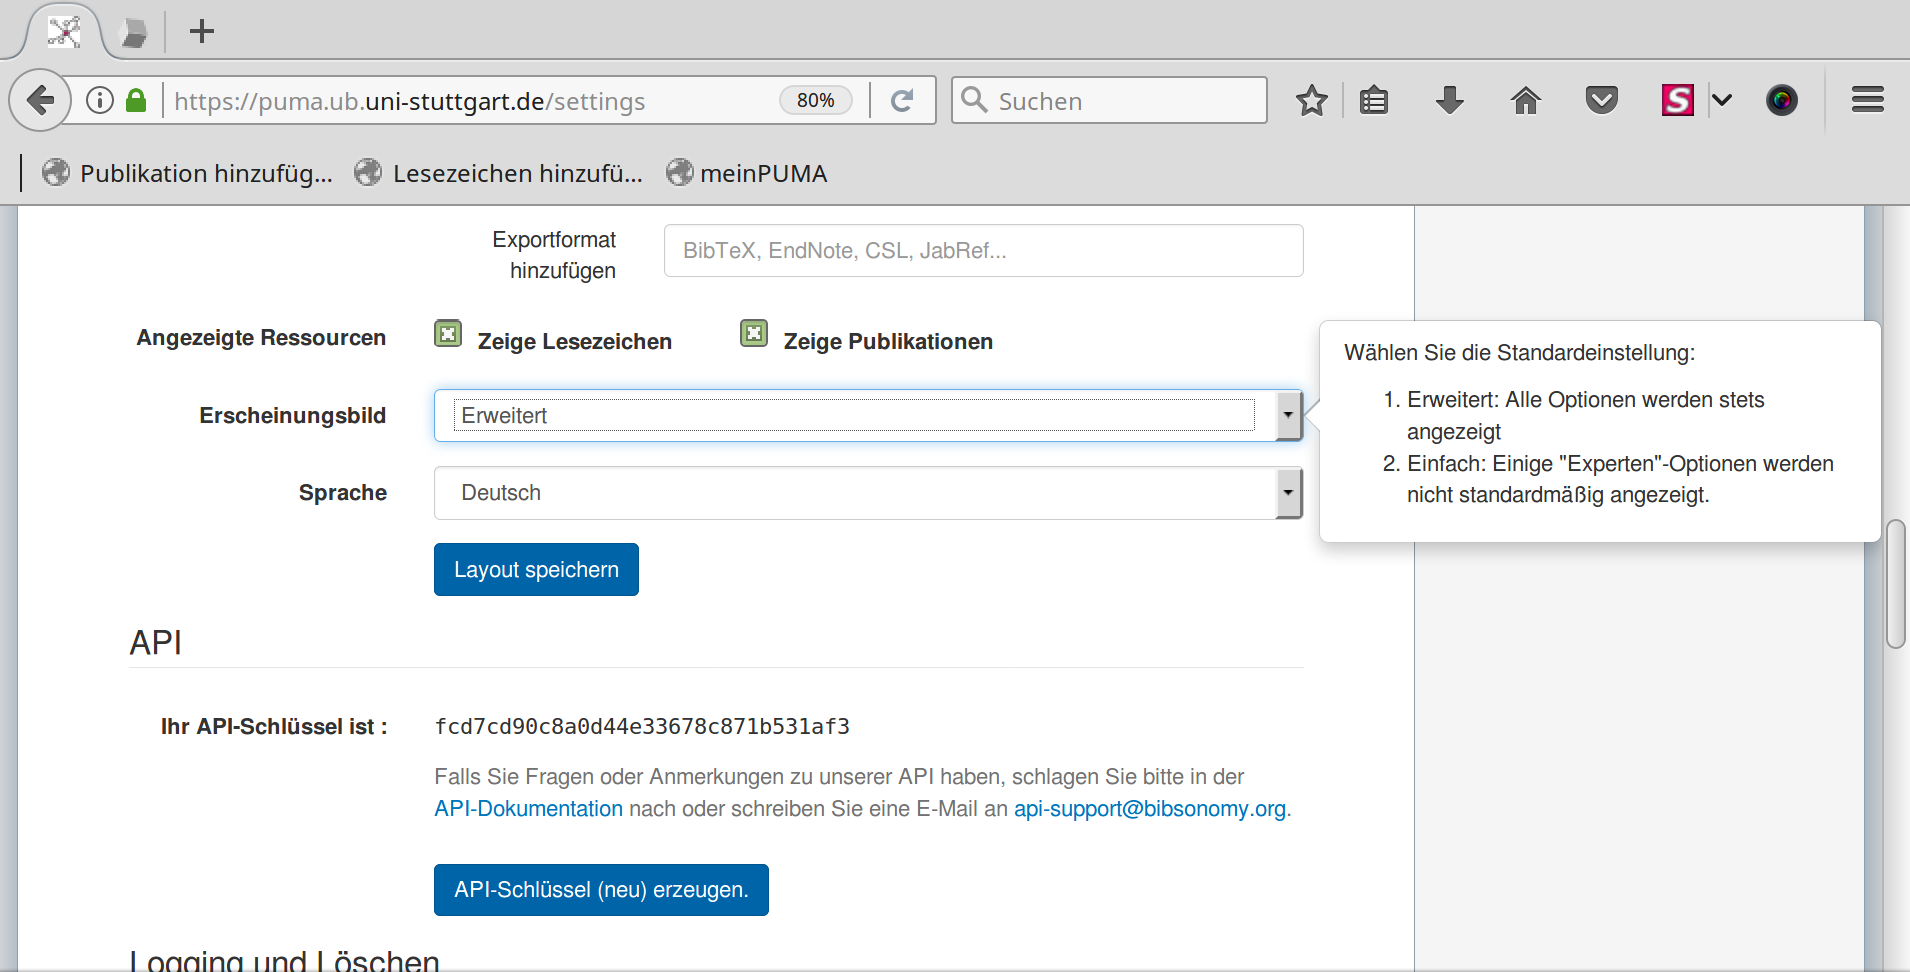
\includegraphics[width=11cm]{Bilder/Kapitel5/Erweiterte_Funktionen}}
 \caption{Erweiterte Funktionen}
 \label{fig:erweiterteFunktionen}
\end{figure} 
%\section{Lebenslauf}
%\label{sec:cv}
%Über \enquote{meinPuma} $\to$ \enquote{Lebenslauf} kann über das Zahnradsymbol sowohl auf das eigene Profil als auch auf die Einstellungen des Layouts (~\hyperref{subseceigenesLayout}) des Lebenslaufs zugegriffen werden. Das eigene Profil kann mit persönlichen Informationen über den Ort, das Geburtsdatum, Beruf und Institution erweitert werden. Darüber hinaus können die wissenschaftlichen Interessen und Hobbies eingetragen werden. Publikationen und Lesezeichen, die mit \tag \textit{<myown />} getaggt werden, erscheinen ebenfalls auf dieser Seite. In den Profileinstellungen kann die Sichtbarkeit dieser Informationen auf privat, für Freunde oder öffentlich sichtbar eingestellt werden. Bei privat sehen andere Nutzer nur den Nutzernamen.
%%\begin{figure}[h!]
 %%\centering
 %%\fbox{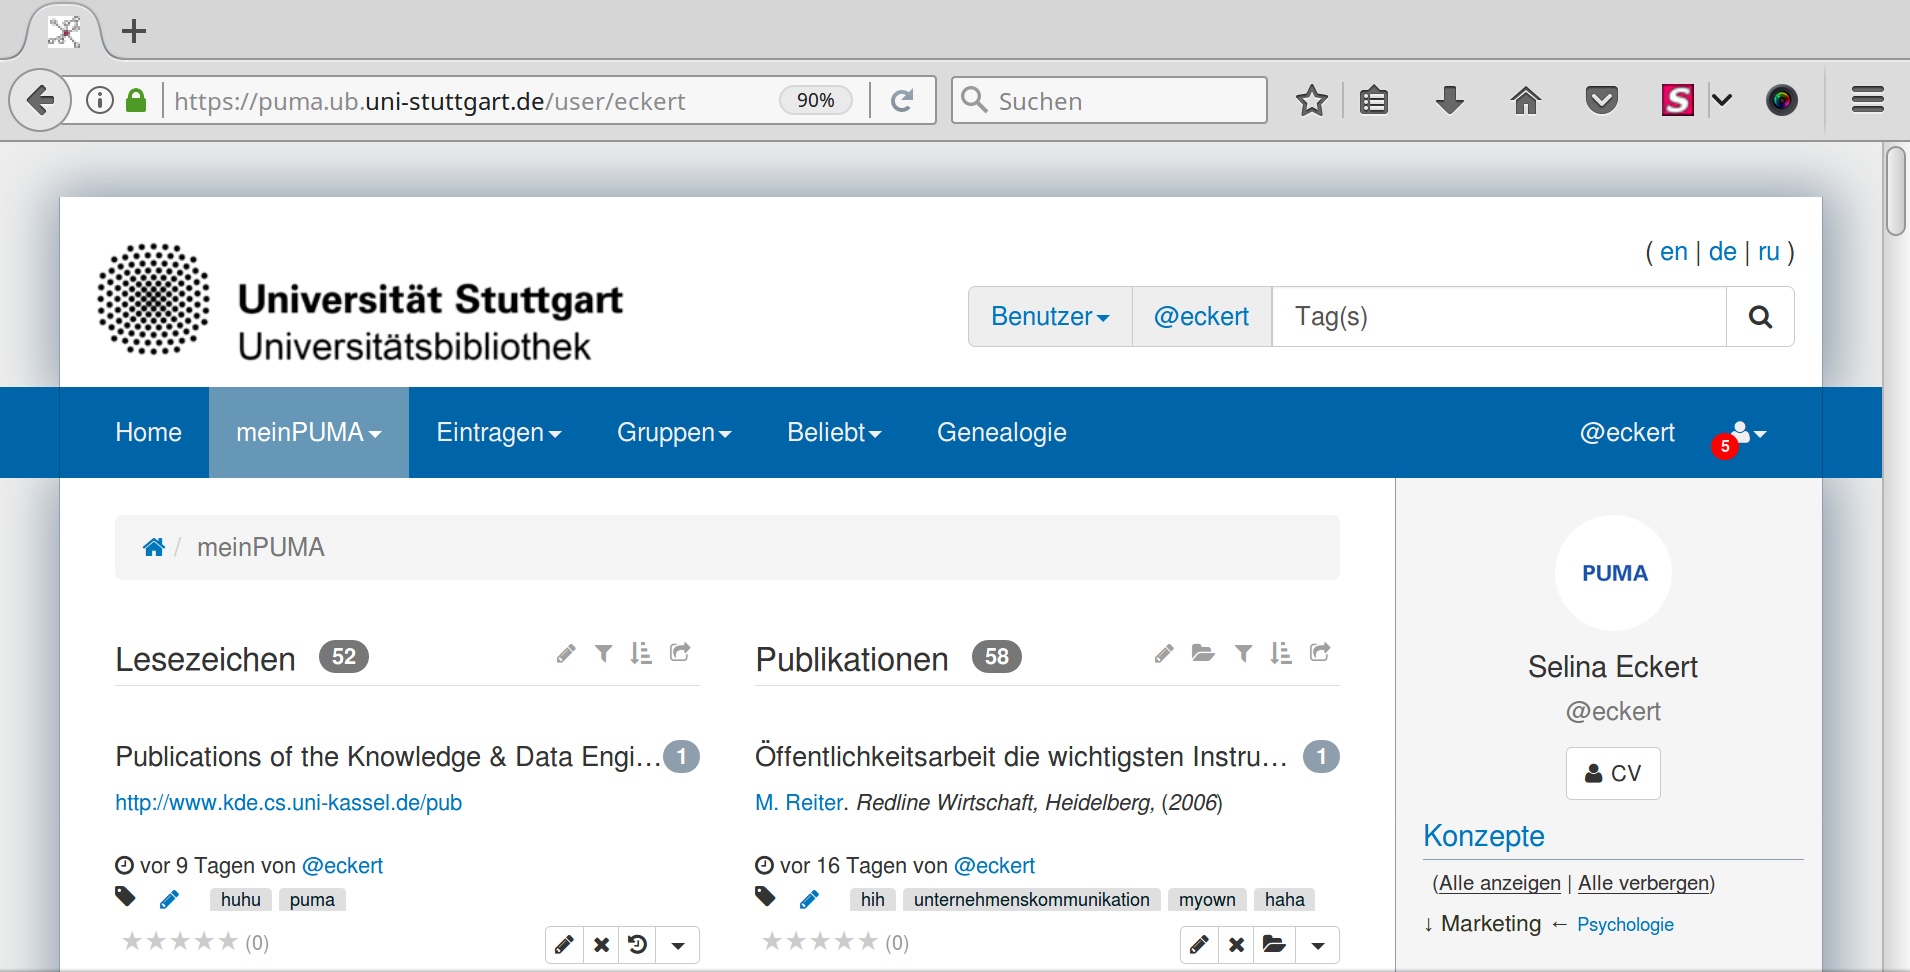
\includegraphics[width=11cm]{Bilder/Kapitel5/CV_Benutzerkonto}}
 %%\caption{Das Benutzerkonto}
 %%\label{fig:benutzerkonto}
%%\end{figure}  
%%Lebenslauf bearbeiten\index{Lebenslauf!bearbeiten}: 
%%\begin{enumerate}
    %%\item Klicken Sie auf Ihren Benutzernamen (@username).
    %%\item Klicken Sie rechts neben Ihrem Profilbild auf den CV-Button.
    %%\item Ihr Lebenslauf öffnet sich (Ansicht: So wie ihn andere Nutzer sehen).
    %%\item Um den Lebenslauf zu bearbeiten klicken Sie auf das schwarze Zahnrad neben \enquote{Curriculum Vitae}.
    %%\item Klicken Sie anschließend im Untermenü auf \enquote{Lebenslauf bearbeiten}. Sie können nun ein vordefiniertes Layout auswählen oder selbst ein Layout mit der MediaWiki-Syntax definieren.
%%\end{enumerate}
%%\textbf{Alternativer Weg:} 
%%\begin{enumerate}
    %%\item Klicken Sie auf das Personensymbol. Es öffnet sich ein Untermenü.
    %%\item Klicken Sie im Untermenü auf \enquote{Einstellungen}.
    %%\item Eine neue Seite öffnet sich. Klicken Sie auf den Reiter \enquote{Lebenslauf}. Sie können nun ein vordefiniertes Layout auswählen oder selber ein Layout mit der MediaWiki-Syntax definieren.
%%\end{enumerate}
%%\begin{wrapfigure}{l}{5cm}
%\begin{mdframed}[style=tipp]\texttt{Wenn Sie zwischen den vordefinierten Layouts wechseln, geht Ihr selbst definiertes Layout verloren.} \
%\end{mdframed}
%\todo{vielleicht zwei Styles Achtung und Tipp: Bin insgesamt mit dem Layout dieser Kästen nicht zufrieden}
%%\end{wrapfigure}
%\begin{figure}[h!]
 %\centering
 %\fbox{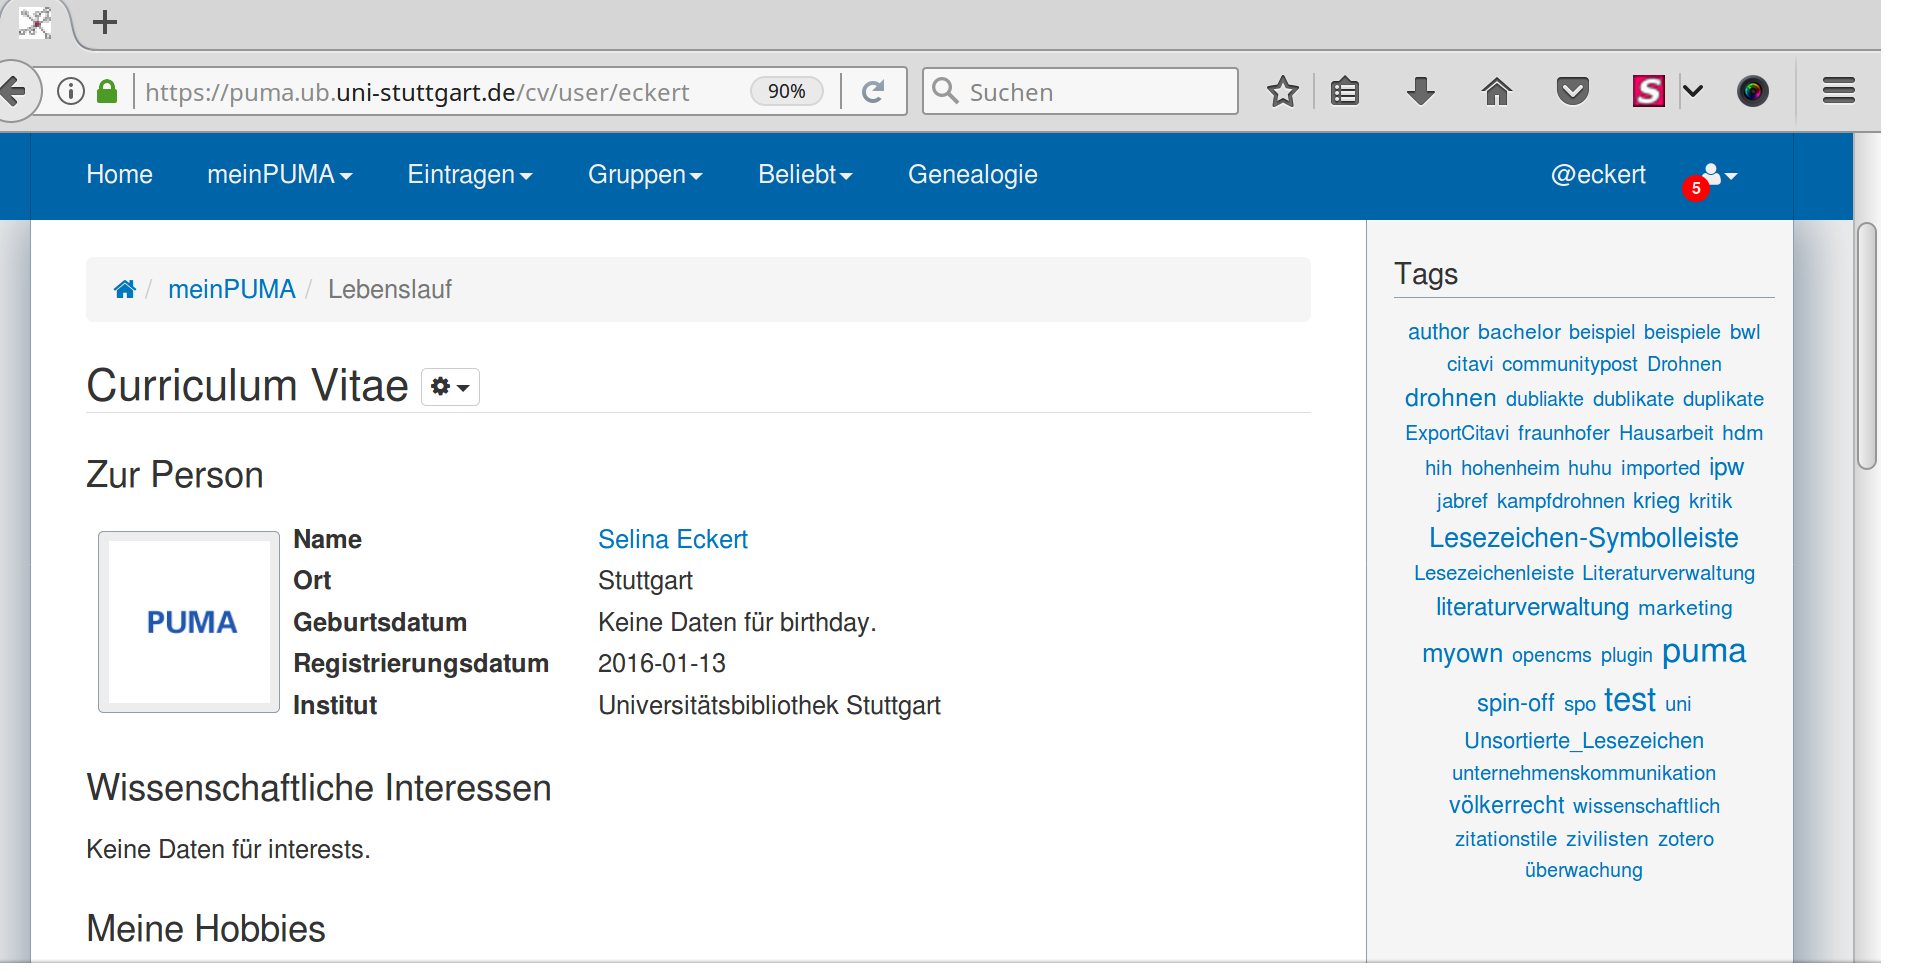
\includegraphics[width=11cm]{Bilder/Kapitel5/CV_Seite}}
 %\caption{Curriculum Vitae-Seite}
 %\label{fig:curriculumVitaeSeite}
%\end{figure}
%\todo[inline]{Bild ist veraltet, neuen Screenshot}
%\subsection{Eigenes Layout\index{Lebenslauf!Eigenes Layout}:}
%\label{subsec:eigenesLayout}
%Um sich selbst ein Layout zu definieren, wird die MediaWiki-Syntax verwendet. Dazu gibt es einige XHTML-Tags:
%\begin{figure}[h!]
 %\centering
 %\fbox{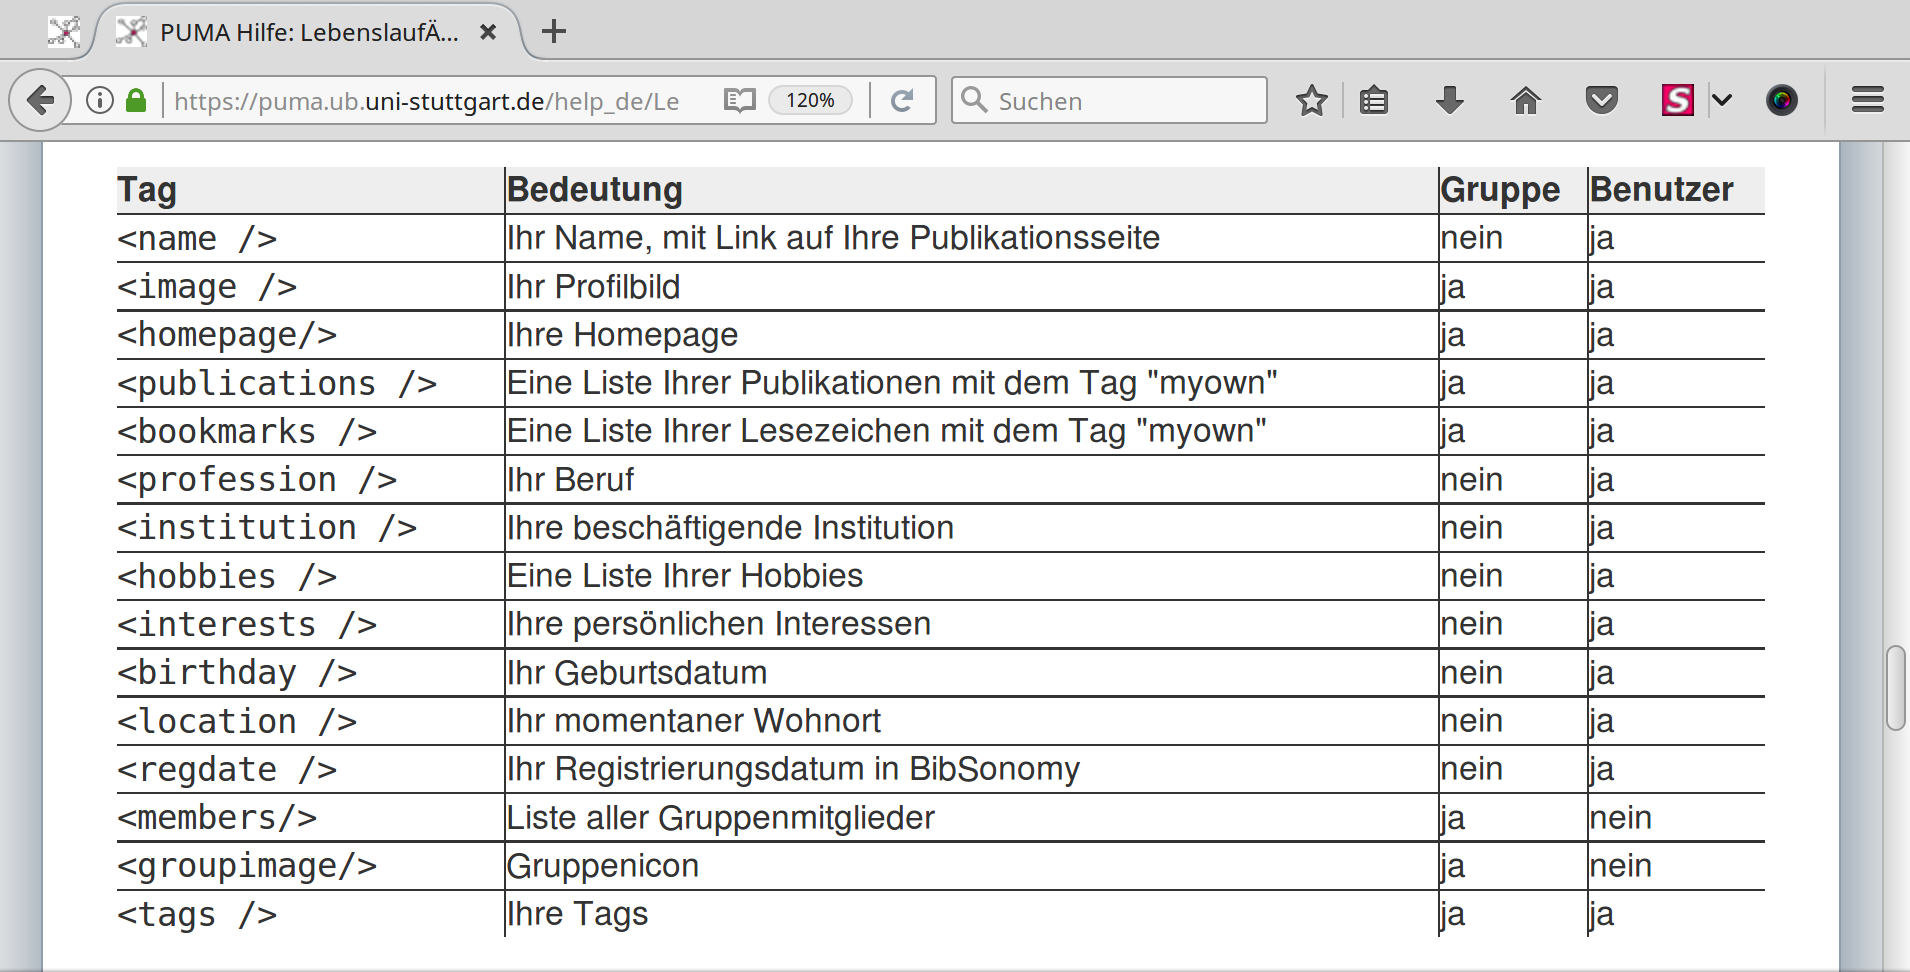
\includegraphics[width=11cm]{Bilder/Kapitel5/xhtml_tags}}
 %\caption{XHTML-Tags}
 %\label{fig:xhtmlTags}
%\end{figure} % Tabelle % ist XHTML bei wiki???
%\newline
%Für die Publikations- und Lesezeichenanzeige können außerdem zusätzliche Tags angegeben werden, um diese aus der eigenen Sammlung im Lebenslauf anzeigen zu lassen. Beispielsweise liefert \textit{<publications tags=\enquote{data mining} />} alle Publikationen, die sowohl mit data als auch mit mining getaggt wurden.  
\todo[inline]{Eigener Abschnitt zu Lebenslauf auskommentiert, ist das wirklich nötig? Eventuell noch oben ergänzen}
\section{Publikationen und Lesezeichen verwalten}
\label{sec:publikationen}
 Mit PUMA können sowohl Publikationen als auch Lesezeichen verwaltet werden. Es gibt verschiedene Wege Publikationen und Lesezeichen in PUMA einzutragen. Jede Publikation bzw. jedes Lesezeichen benötigt mindestens ein \tag. Mit Hilfe dieser \tags  werden die Einträge kategorisiert. Grundsätzlich sind alle Einträge öffentlich. Öffentliche Einträge sind auch für nicht angemeldete Nutzer sichtbar. Die Sichtbarkeit kann auf privat oder andere (Gruppen oder Freunde) eingeschränkt werden. 
\subsection{Publikationen}
\begin{figure}[htb]
 \centering
 \fbox{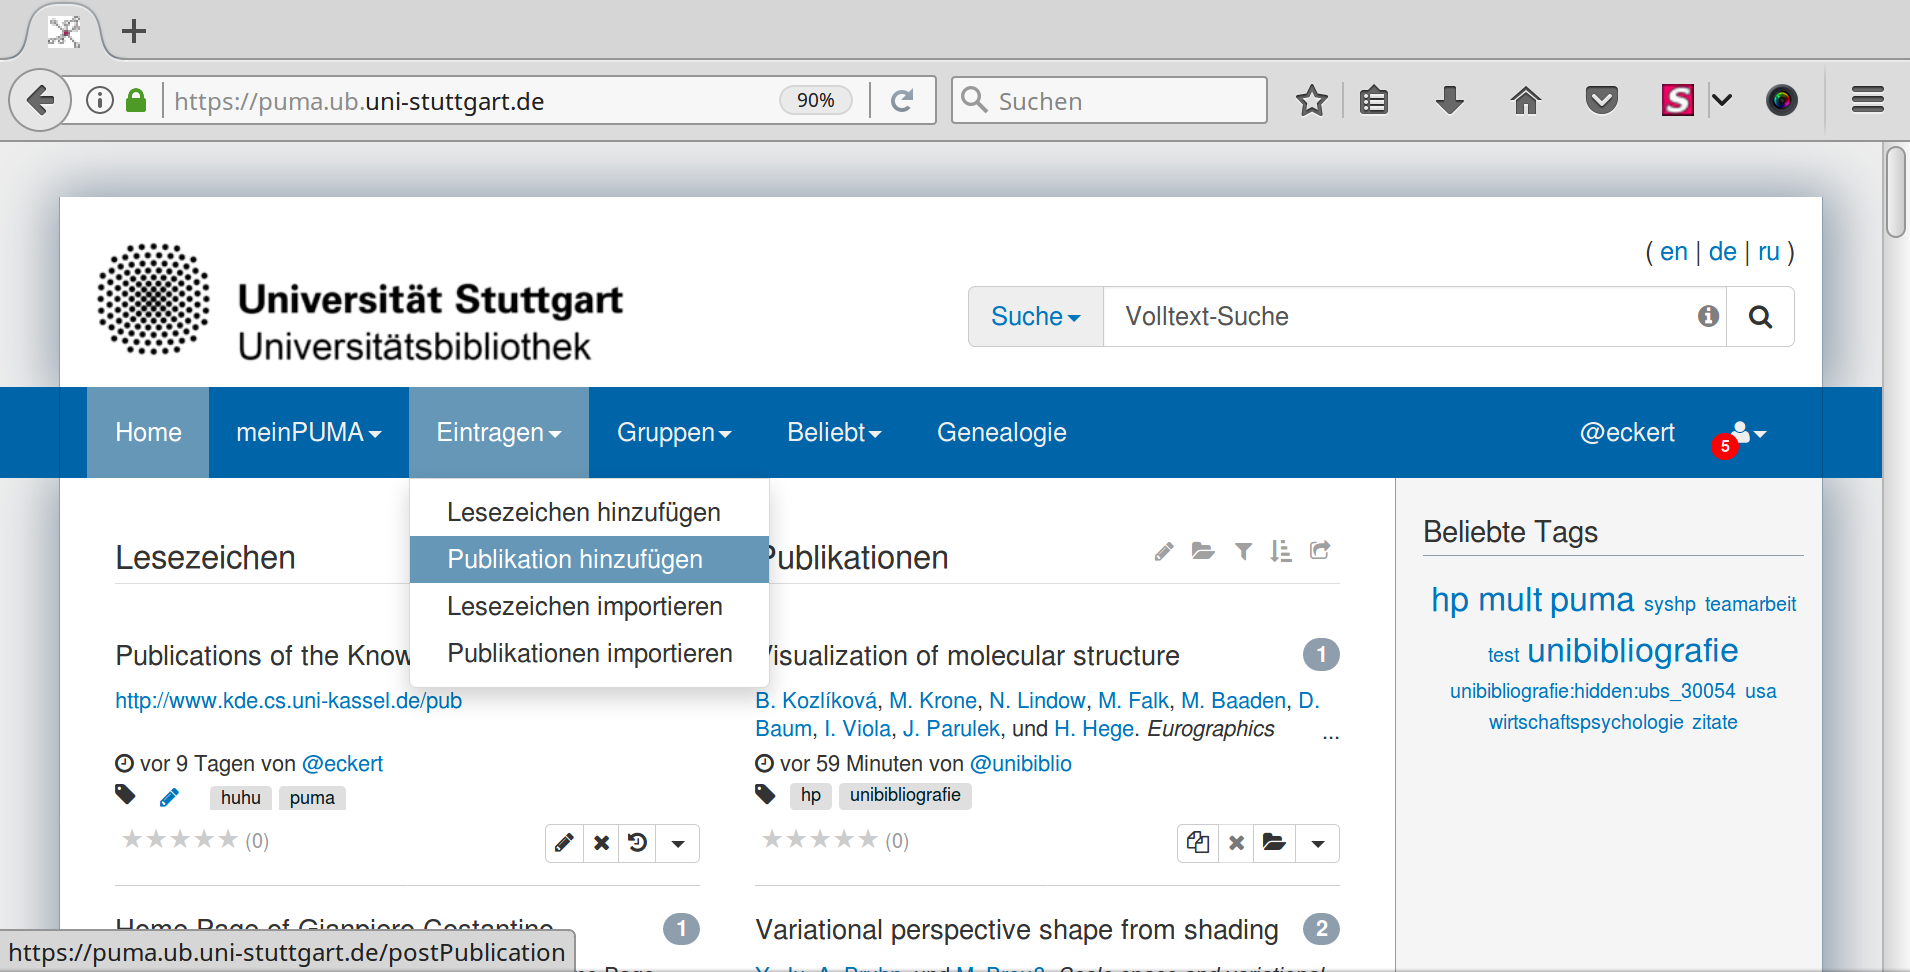
\includegraphics[width=11cm]{Bilder/Kapitel5/Publikation_eintragen}}
 \caption{Publikationen hinzufügen}
 \label{fig:publikationenHinzufügen}
\end{figure}  
Unter dem Menü \enquote{Eintragen} $\to$ \enquote{Publikation hinzufügen}\index{Publikationen!hinzufügen} kann direkt in das Textfeld der Titel oder die ISBN/~ISSN/~DOI der Publikationen eingeben werden. Des Weiteren gibt es zusätzliche Möglichkeiten Publikationen einzutragen:
%\begin{figure}[h!]
 %\centering
 %\fbox{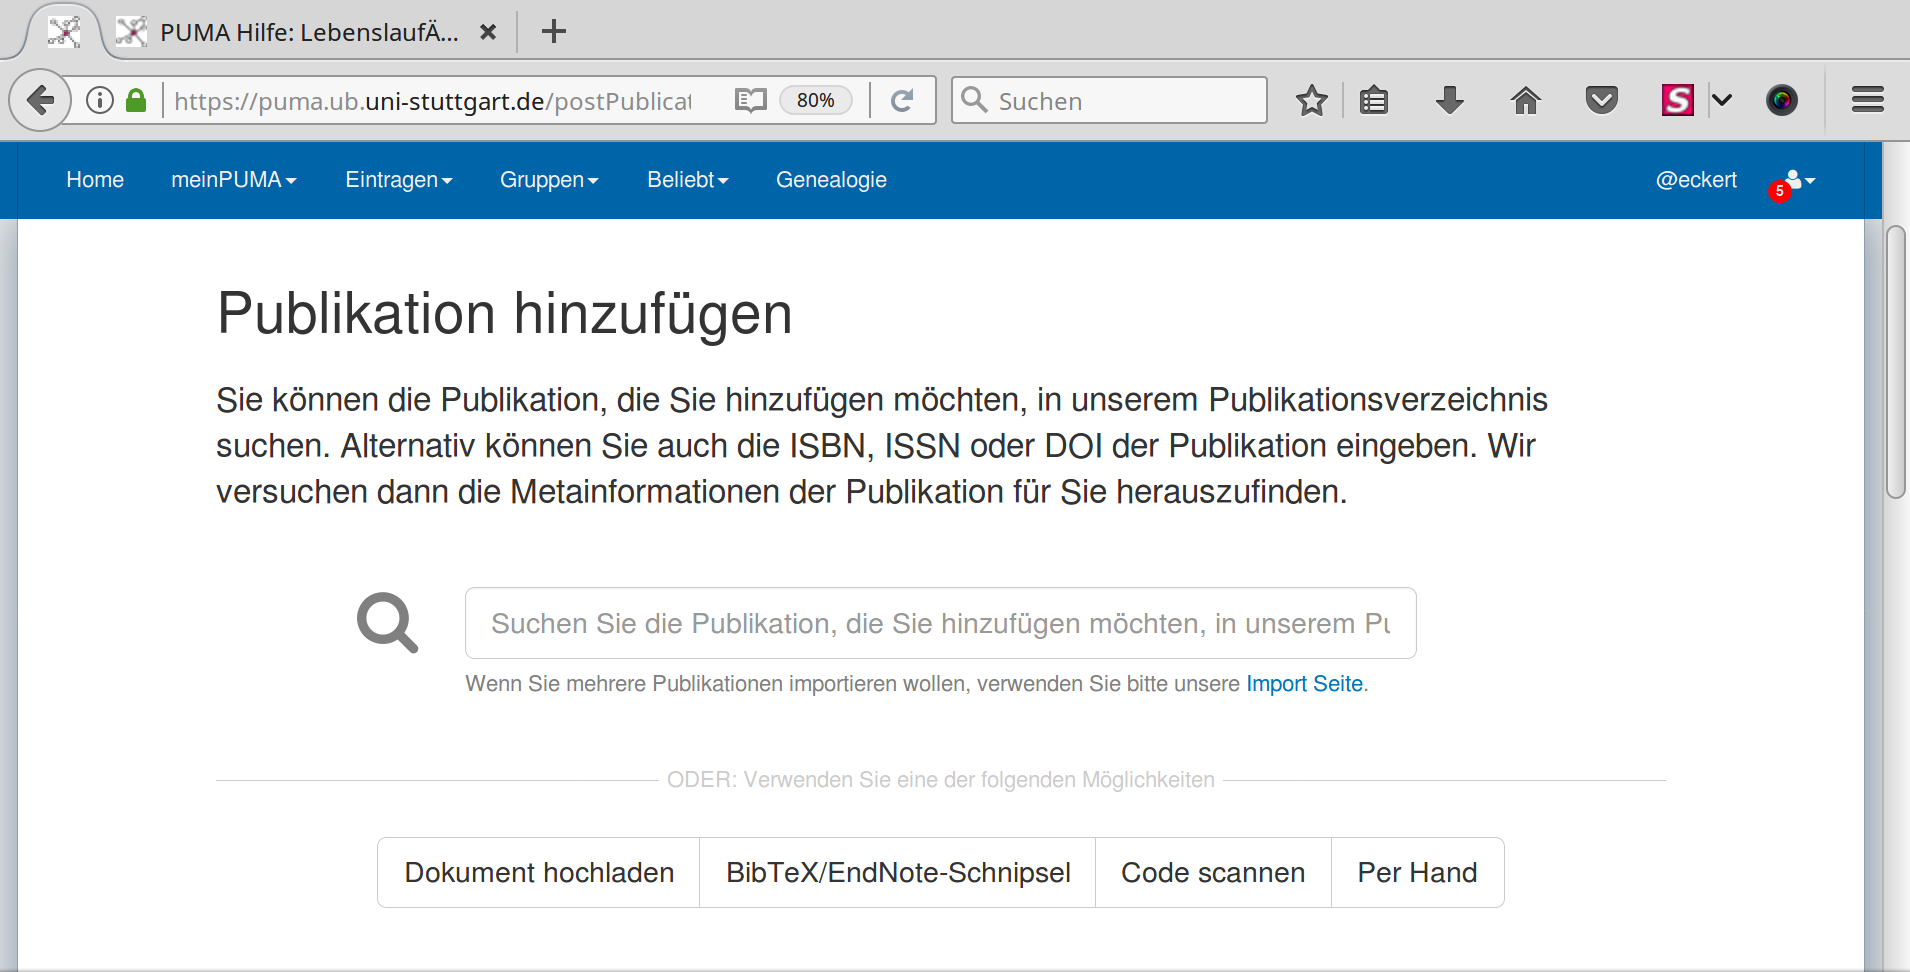
\includegraphics[width=11cm]{Bilder/Kapitel5/Eintragsmoeglichkeiten}}
 %\caption{Eintragsmöglichkeiten}
 %\label{fig:eintragungsmoeglichkeiten}
%\end{figure}  
    \begin{itemize}
    	\item Dokument hochladen:\newline
        Der Volltext einer Publikation kann hier hochgeladen werden. Das übliche Formular zum Eintragen (mit dem hoch geladenen Volltext) der Publikationen öffnet sich. Einige Felder sind bereits ausgefüllt und können ergänzt werden.
				\begin{tip}
Achtung Betaversion! Diese Funktion befindet sich gerade in der Entwicklung.
\end{tip}
			\item BibTex\index{BibTex}/EndNote\index{EndNote}-Schnipsel:\newline
			Kopierte Zitationen können hier eingefügt werden. Diese Informationen werden dann übernommen und können ergänzt werden.
        \item Code scannen\index{Code Scannen}: \newline
Über eine Webcam kann der Barcode gescannt werden. Ggf. muss der Zugriff von PUMA auf die Webcam erlaubt werden. Sobald der Barcode erkannt wurde, werden die Daten angezeigt und können ergänzt werden
        \item Per Hand:
				Hier kann der Eintragstyp, Titel, Autor(en), Herausgeber und Jahr der Publikation eingetragen werden. Mit \enquote{Weiter} erscheinen alle Felder der Eingabemaske. \todo{Verweis auf Eintragstypen}
    \end{itemize}
\begin{tip} Über die Url \url{https://puma.ub.uni-stuttgart.de/editPublication} kann direkt auf die erweiterte Eingabemaske zugegriffen werden
\end{tip}		
%\begin{figure}[h!]
 %\centering
 %\fbox{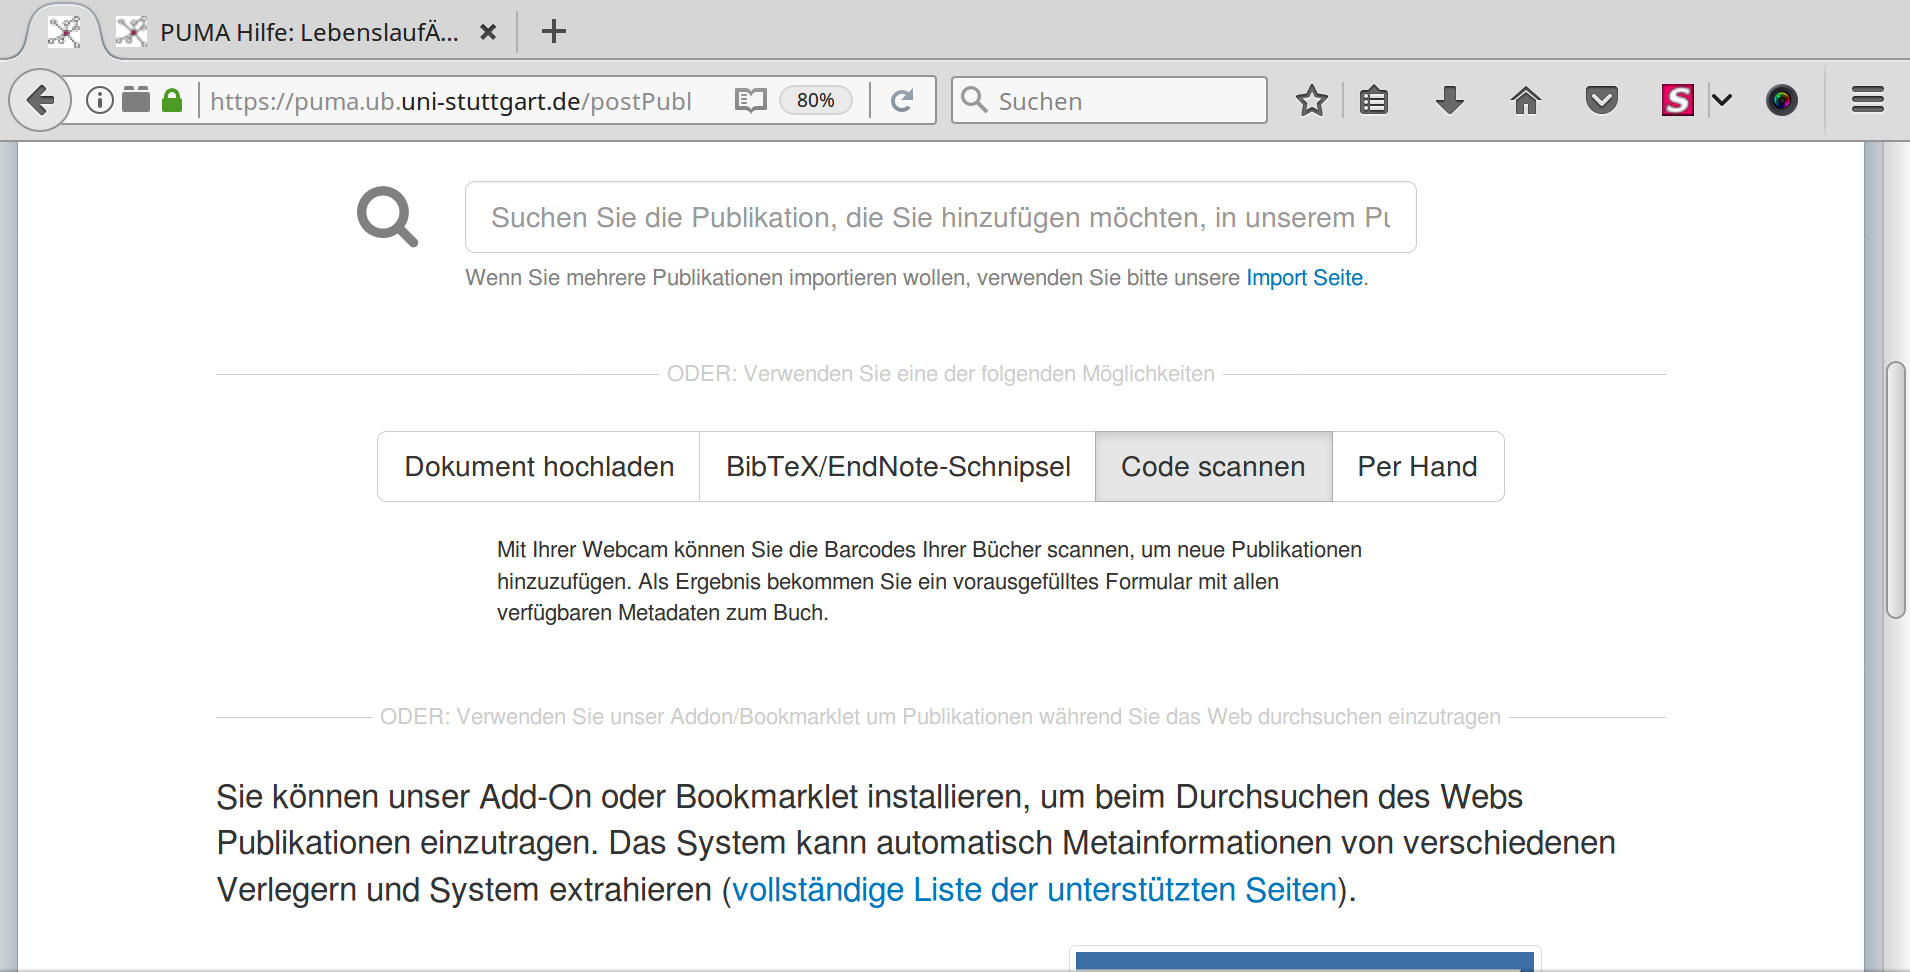
\includegraphics[width=11cm]{Bilder/Kapitel5/Code_scannen}}
 %\caption{Code scannen}
 %\label{fig:codeScannen}
%\end{figure}
Über \enquote{Eintragen} $\to$ \enquote{Publikation importieren} kann eine Text-Datei hochgeladen werden. Folgende Aktionen können bei den Einträgen der Datei in PUMA ausgewählt werden:
\begin{tip}
Bei EndNote wird beim Speichern eine Datei mit der Endung .enl erzeugt, diese enthält die komplette Datenbank. Für den Import in PUMA sollte ein Textdatei importiert werden. Dazu muss die Datei in EndNote nicht speichern, sondern exportieren. PUMA kann mit verschiedenen Formaten umgehen. Um BibTex zu exportieren muss der Output-Stil angepasst werden. Wenn BibTex nicht angezeigt wird, unter \enquote{Edit} $\to$ \enquote{Output-Styles} $\to$ \enquote{Open Style Manager} BibTex aus der Liste auswählen. Über \enquote{File} $\to$\enquote{Export} den \enquote{BibTex Export} auswählen. Beim Speichern \enquote{Text only} auswählen und die Datei mit der Endung .bib speichern.
\end{tip}
Nach dem Hochladen stehen verschiedene Möglichkeiten zur Verfügung die Einträge weiter zu bearbeiten:
\begin{itemize}
\item Tags zu allen ausgewählten Einträgen hinzufügen: An jeden Eintrag wird der gleiche \tag hinzugefügt
\item Die Tags aller ausgewählten Einträge separat bearbeiten: \tags können auch an einzelne Einträge hinzugefügt werden
\item BibTeX-Schlüssel normalisieren: BibTex-Schlüssel werden nach dem Schema NameJahrTitel normalisiert, wobei Name der Nachname des primären Autors , Jahr das Jahr der Veröffentlichung und Titel das erste Wort des Titels der Publikation ist, das mehr als fünf Buchstaben enthält. Beispiel: knuth1998programming.
\item Sichtbarkeit einstellen: öffentlich, privat oder für Freunde \todo{referenz und erklärung ergänzen}
\end{itemize}
\begin{tip} Einträge, die bereits in der eigenen Sammlung vorhanden sind, werden als Fehler angezeigt. Wenn alte Einträge überschrieben werden sollen, kann dies vor dem hochladen der Datei ausgewählt werden.
\end{tip}

\begin{figure}[h!]
 \centering
 \fbox{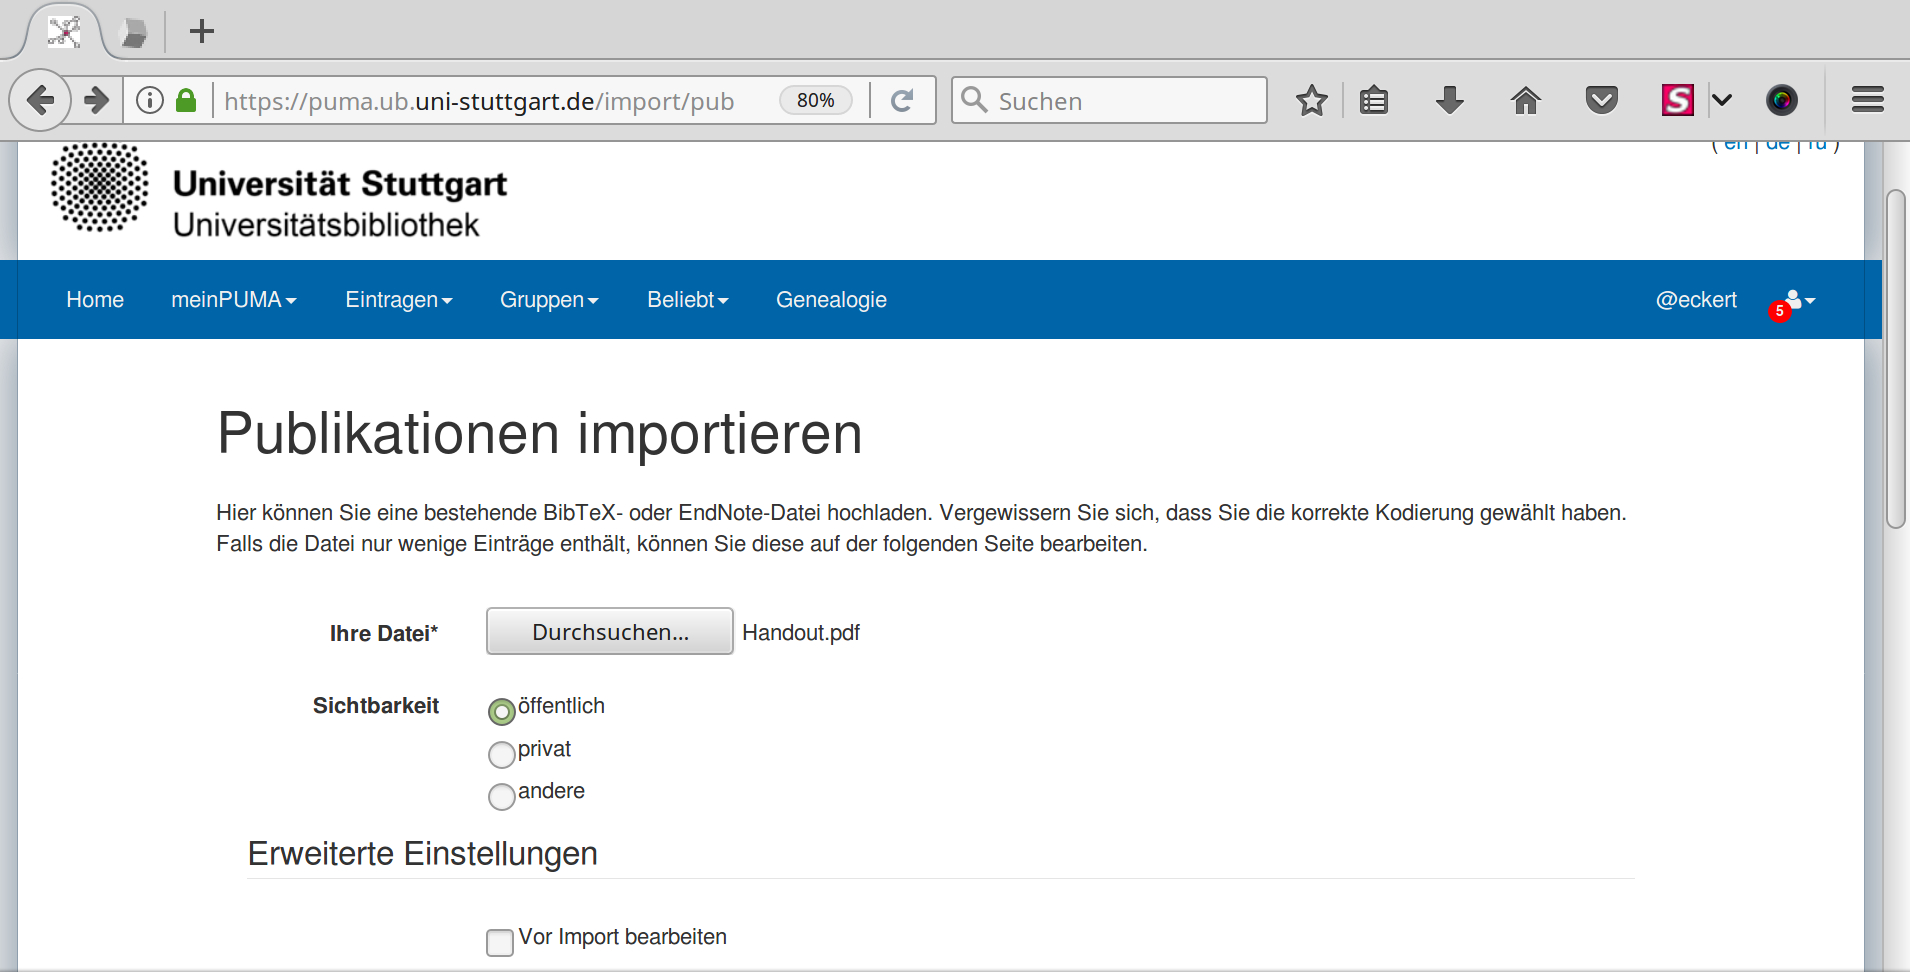
\includegraphics[width=11cm]{Bilder/Kapitel5/Publikationen_importieren}}
 \caption{Publikationen importieren}
 \label{fig:publikationenImportieren}
\end{figure}

\subsection{Lesezeichen} % 2Screenshots: Anfang+Möglichkeiten
\label{subsec:lesezeichen}
Die URL eines Lesezeichen \index{Lesezeichen!hinzufügen} kann über den Menüpunkt \enquote{Eintragen} $\to$ \enquote{Lesezeichen hinzufügen} hinzugefügt werden. 
\begin{figure}[h!]
 \centering
 \fbox{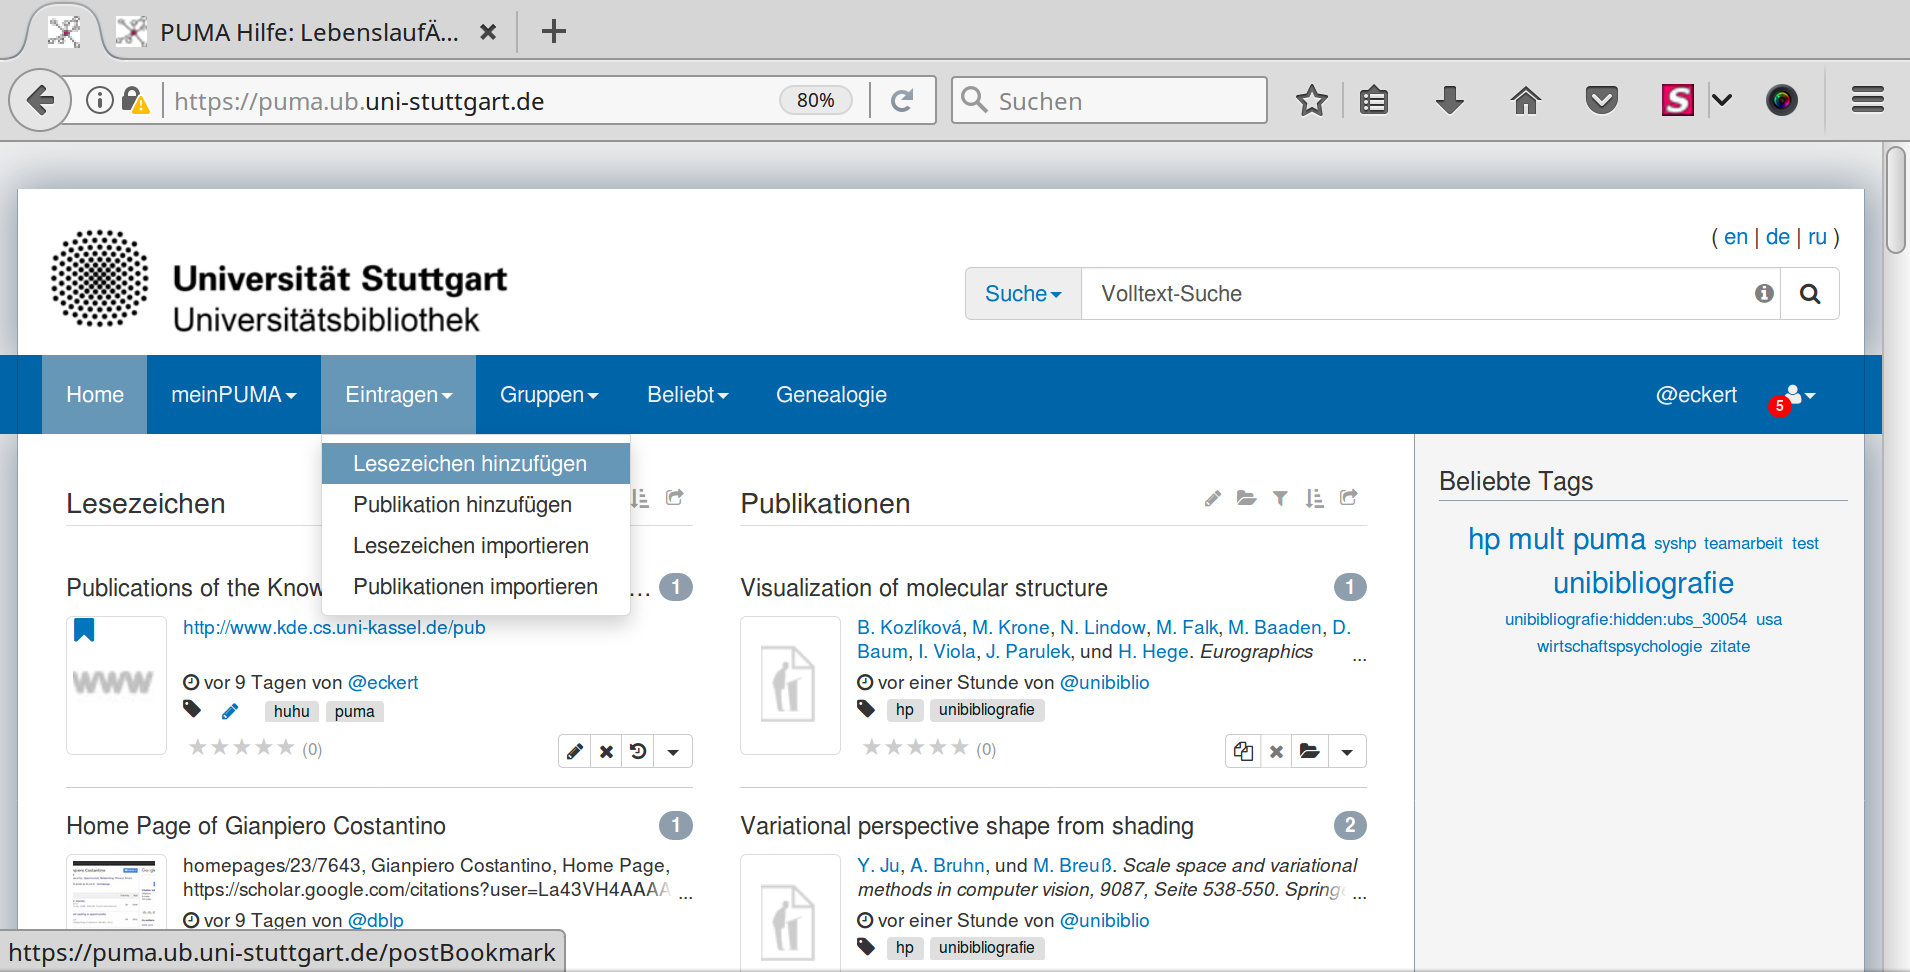
\includegraphics[width=11cm]{Bilder/Kapitel5/Lesezeichen_hinzufuegen}}
 \caption{Lesezeichen hinzufügen}
 \label{fig:lesezeichenHinzufuegen}
\end{figure}  
\underline{Wichtig bei der Recherche und Archivierung von Lesezeichen:}
\begin{itemize}
    \item Puma speichert nicht das eigentliche Dokument, sondern nur die Adresse des Internet-Dokuments. Eine gespeicherte Version der Seite, kann über das Kreis-Pfeilsymbol rechts unter dem Eintrag erreicht werden.
    \item In der Literaturangabe zu einem Internet-Dokument sollte immer das Datum des letzten Abrufs mit angegeben werden. Folgende Möglichkeiten bieten sich an dies in der Literaturliste anzupassen: Die Lesezeicheneinträge werden beim BibTeX-Export als \enquote{electronic} exportiert. Entweder diese Liste für die Literaturangaben manuell im Dokument anpassen, im dem man das \enquote{added-on} Feld in das Bibtex-Feld \enquote{urldate} umbenennt und das Datum im Format xx.yy.zzzz eingibt. \autocite[Vgl. das Benutzerhandbuch zum BibLaTeX Paket][S.10 (der Eingabetyp \enquote{online} wird synonym zu \enquote{electronic} verwendet. Damit der Zitationsstil das Abrufdatum hinzufügt muss das Feld urldate ausgefüllt sein.)]{lehmann2016biblatex} Dann bei den Publikationen wieder exportieren. Man kann auch gleich beim Sammeln der Lesezeichen diese sowohl bei den Lesezeichen als auch bei den Publikationen eintragen. Bei PUMA muss immer ein Autor oder Herausgeber und das Jahr ausgefüllt werden. Die meisten Zitationsstile unterdrücken den Editor bei der Ausgabe (Vgl. \todo{Zitiertips schreiben und verweisen})
    \item PUMA unterstützt die RFC 7089\footnote{\url{http://tools.ietf.org/html/rfc7089}} Spezifikation\index{RFC 7089 Spezifikation}. Damit wird es möglich, Lesezeichen so zu betrachten, wie sie in PUMA gespeichert wurden, selbst wenn sich die Seite in der Zwischenzeit geändert hat. Um diese Funktion zu nutzen, müssen Sie das Memento-Plugin in ihrem Browser installieren. Das Plugin existiert für Mozilla Firefox\footnote{\url{https://addons.mozilla.org/de/firefox/addon/mementofox/}} und Google Chrome\footnote{\url{https://chrome.google.com/webstore/detail/memento-time-travel/jgbfpjledahoajcppakbgilmojkaghgm?hl=en&gl=US}}. \todo{auf Marios anwort warten}
\end{itemize}
\section{Versionierung der Publikationen und Lesezeichen}
\label{sec:versionierung}
Publikationen und Lesezeichen können jederzeit eingetragen und bearbeitet werden. Um sich einen Überblick über die vorgenommen Änderungen zu verschaffen, bietet PUMA eine Versionsgeschichte\index{Versionierung} zu jeder Publikation und jedem Lesezeichen an. Dazu in der eigenen Sammlung auf den kleinen schwarzen Pfeil neben einer beliebigen Publikation klicken. Es öffnet sich ein Dropdown-Menü, in dem \enquote{Versionsverlauf dieses Eintrags} ausgewählt werden kann. Die verlaufsseite zeigt:
\begin {itemize}
\item das Bearbeitungsdatum
\item die Anzahl der geänderten Felder in jeder Version
\item hinzugefügte (grün) und gelöschte (rot) Textteile
\end{itemize}
\begin{figure}[h!]
 \centering
 \fbox{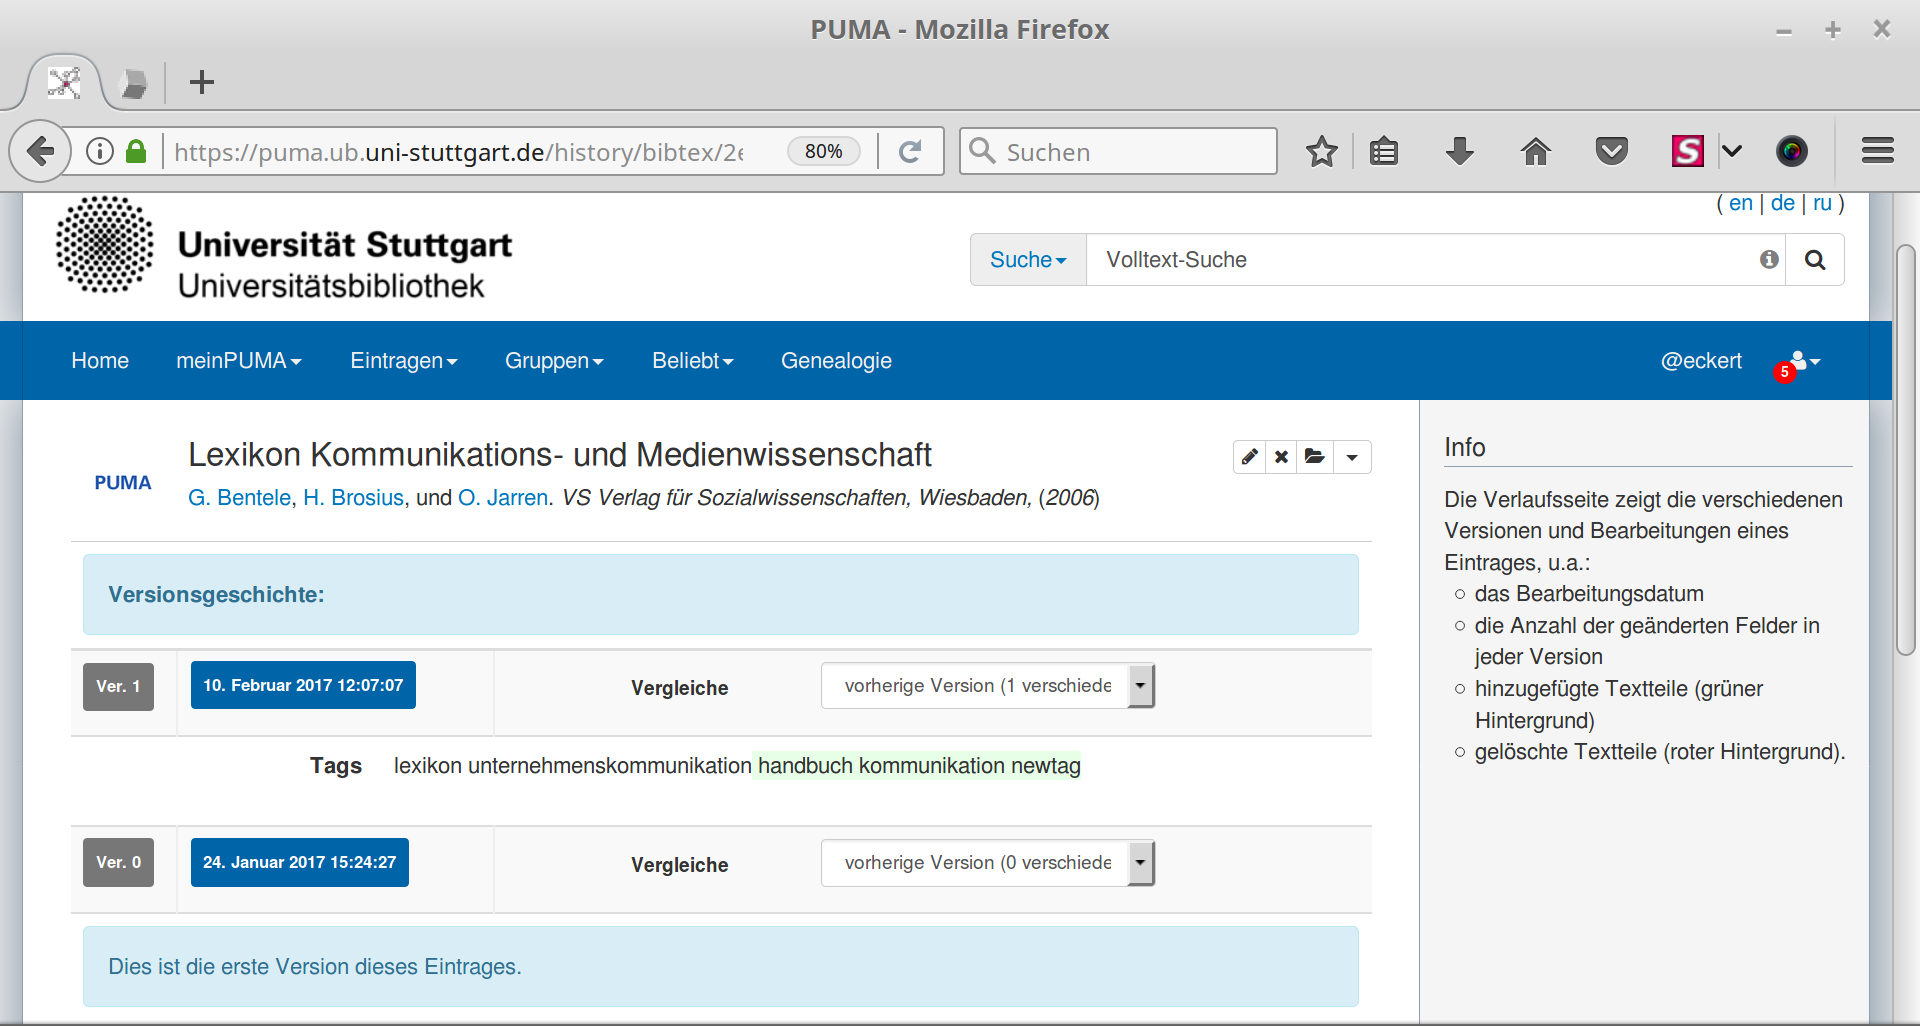
\includegraphics[width=9cm]{Bilder/Kapitel5/Versionsgeschichte}}
 \caption{Die Versionsgeschichte}
 \label{fig:versionsgeschichte}
\end{figure} 
PUMA ermöglicht es HTML-Dateien zu importieren. Hierfür die Lesezeichen aus dem Browser als HTML-Datei exportieren. Über \enquote{Eintrage} $\to$ \enquote{Lesezeichen importieren} die HTML-Datei auswählen und die Sichtbarkeit auf öffentlich oder privat stellen. PUMA erkennt vorhandene Lesezeichen, es kann ausgewählt werden, ob diese überschrieben werden. Um den Import endgültig durchzuführen, mit \enquote{Importieren} bestätigen.Ein \tag wird automatisch vergeben. Weitere \tags müssen manuell hinzugefügt werden. \todo{Verweis ablage und Stapelverarbeitung}
\begin{figure}[h!]
 \centering
 \fbox{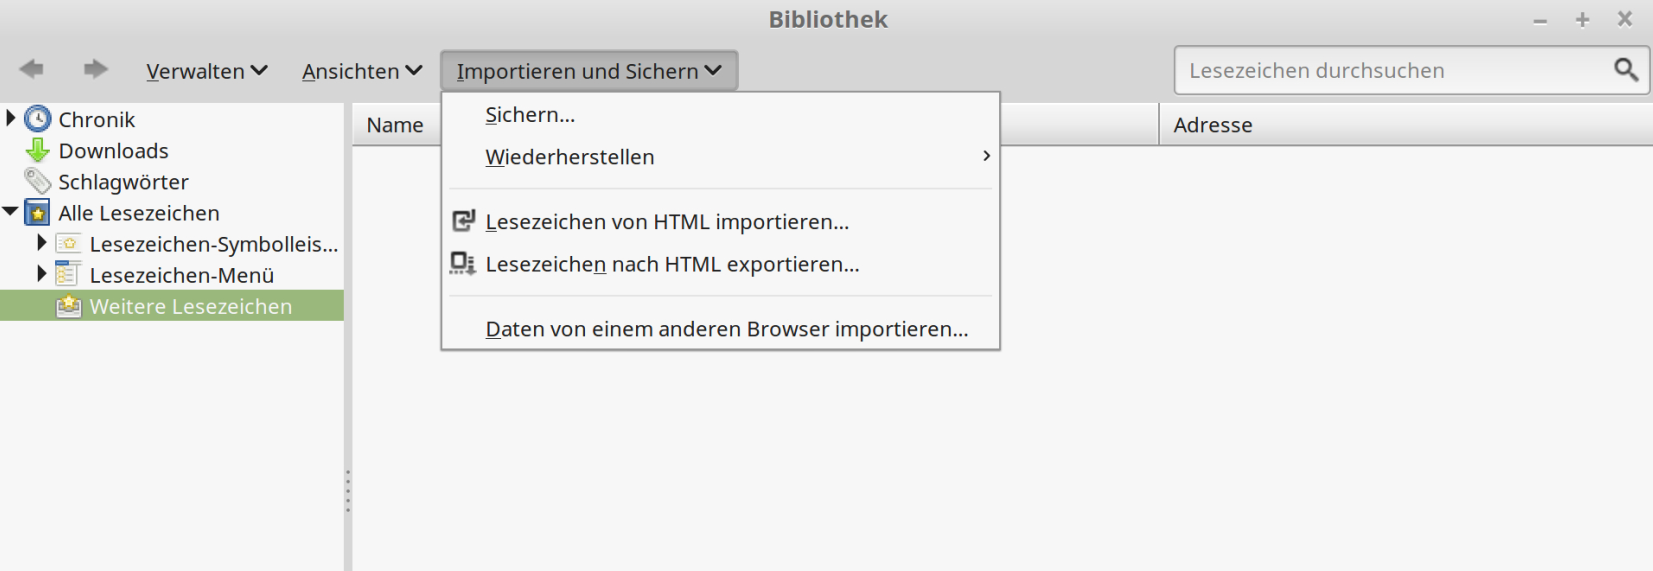
\includegraphics[width=11cm]{Bilder/Kapitel5/Firefox_Importieren_Speichern}}
 \caption{Importieren und Sichern}
 \label{fig:importierenSichern}
\end{figure}
\subsection{HTML-Datei\index{HTML-Datei} in PUMA importieren}
\label{subsec:htmlDateiImportieren}
\begin{figure}[h!]
 \centering
 \fbox{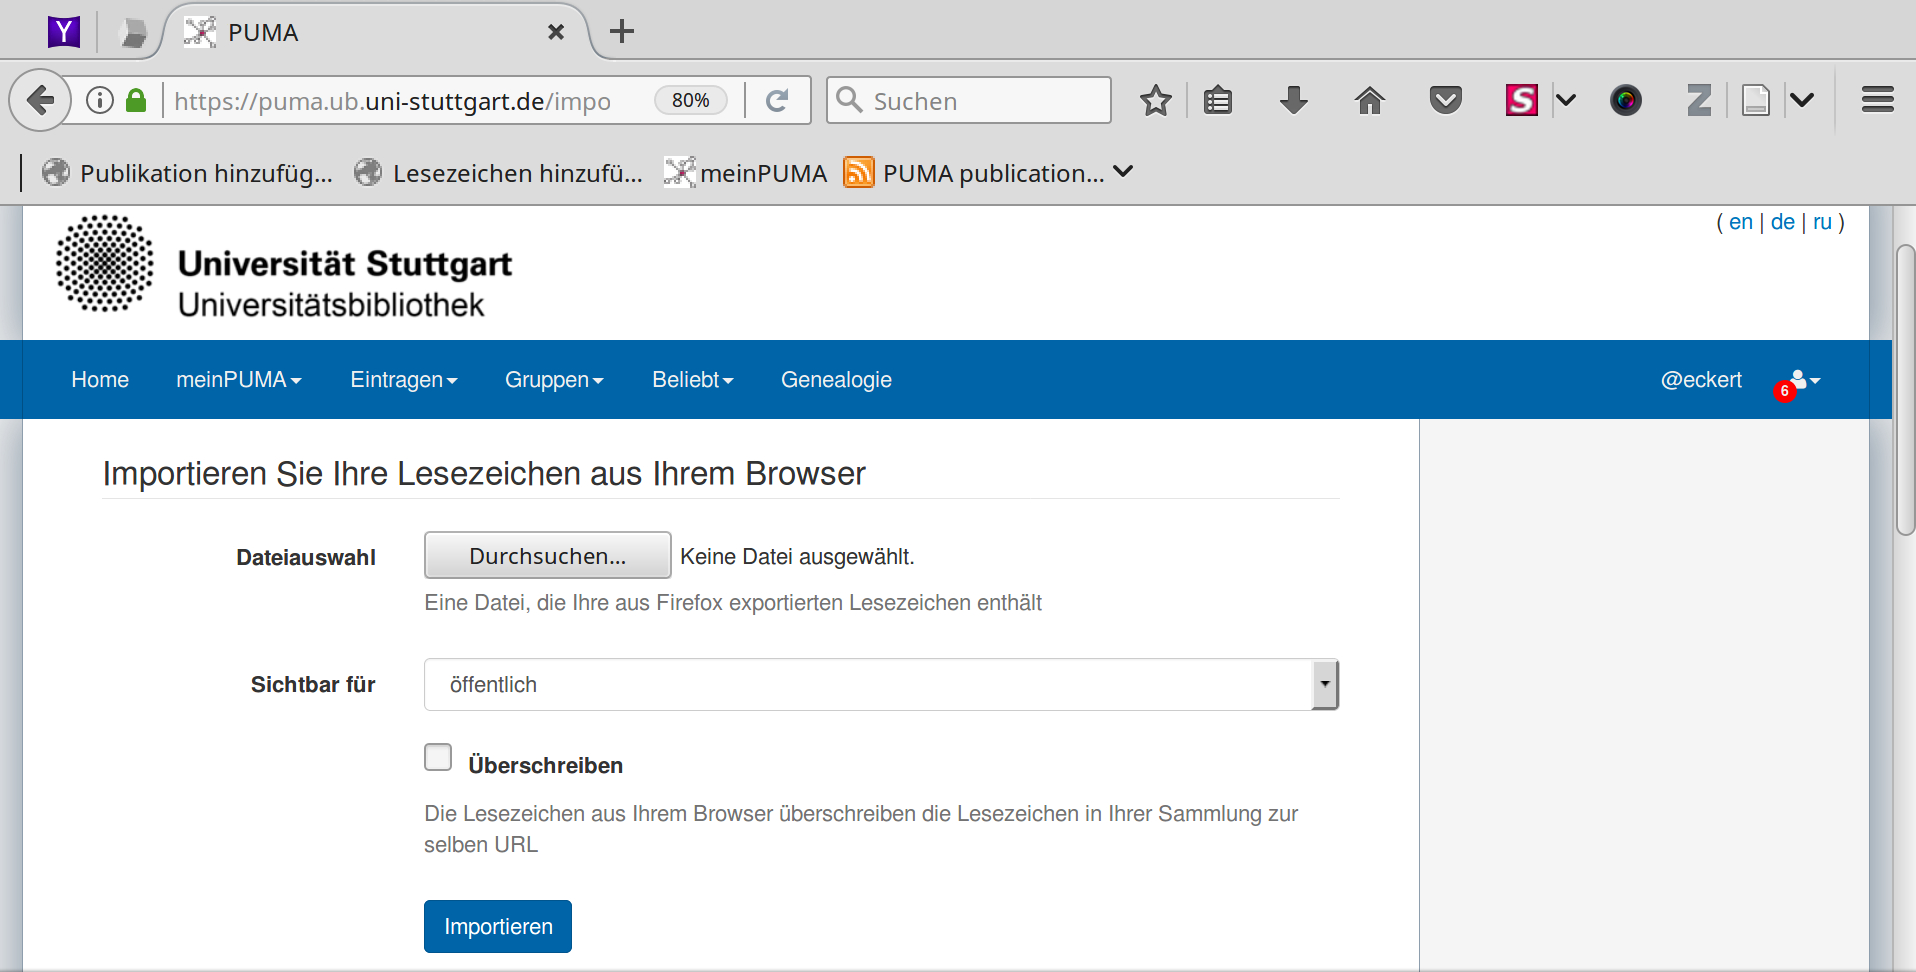
\includegraphics[width=11cm]{Bilder/Kapitel5/HTML-Datei_hochladen}}
 \caption{HTML-Datei hochladen}
 \label{fig:htmlDateiHochladen}
\end{figure}

\textbf{Delicious}
\label{subsec:delicious}
Lesezeichen von Delicious\index{Delicious} können direkt in PUMA importiert werden, dazu statt eine Datei anzugeben, die Delicious-Nutzerdaten im Bereich \enquote{Importieren Sie Ihre Delicious Daten} eingeben. \newline
Es kann gewählt werden, ob Lesezeichen oder Tag-Bundles importieren werden sollen. Bei \enquote{Lesezeichen} werden zusammen mit den Lesezeichen auch die dazugehörigen Tags und Sichtbarkeitsbedingungen mit übernommen.
\begin{figure}[h!]
 \centering
 \fbox{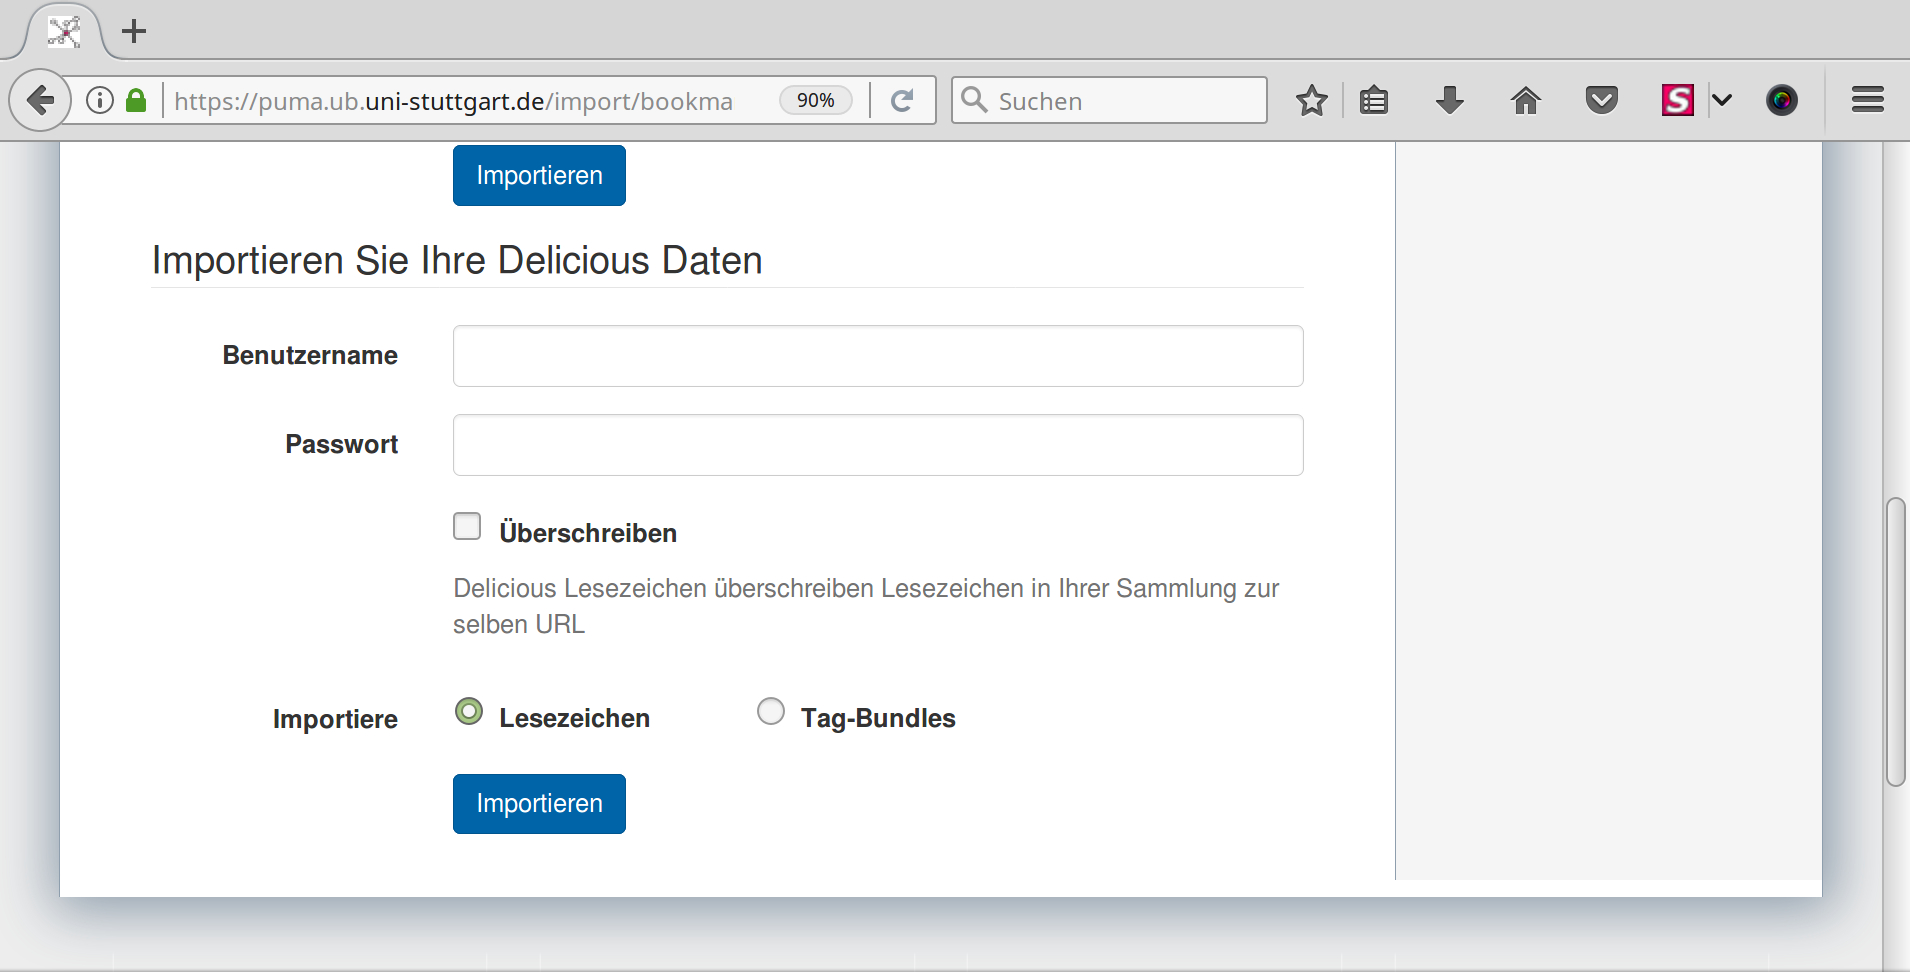
\includegraphics[width=11cm]{Bilder/Kapitel5/Delicious_Daten}}
 \caption{Delicious Daten}
 \label{fig:deliciousDaten}
\end{figure} 

\textbf{Chrome}%Screenshots hab ich schon
\newline Um die Lesezeichen in Chrome\index{Chrome} als HTML-Datei zu exportieren, im Menü oben rechts auf \enquote{Lesezeichen} und anschließend auf \enquote{Lesezeichen-Manager} klicken. Es öffnet sich ein neues Fenster, in dem über \enquote{Organisieren} im Dropdown-Menü \enquote{Lesezeichen in HTML-Datei exportieren...} ausgewählt werden kann.  
\begin{figure}[h!]
 \centering
 \fbox{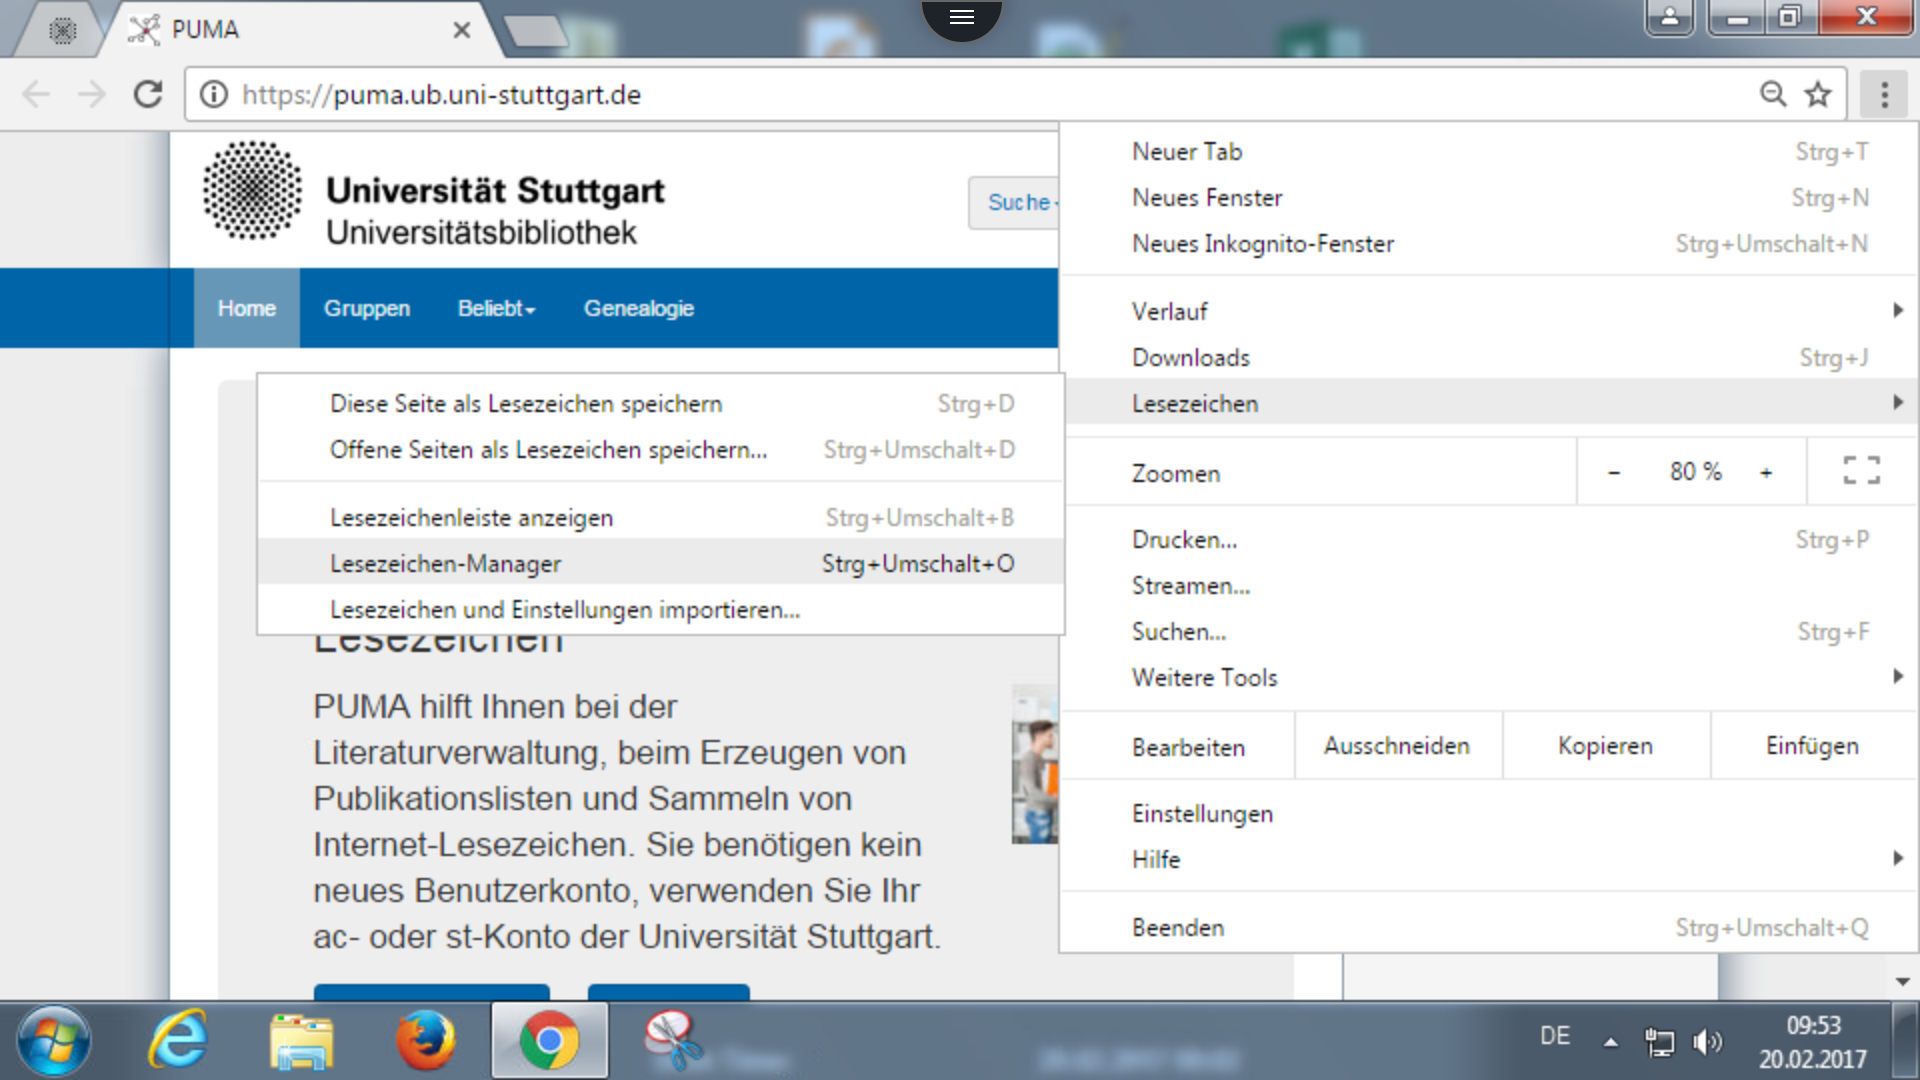
\includegraphics[width=11cm]{Bilder/Kapitel5/Lesezeichen-Manager_Chrome}}
 \caption{Der Lesezeichen-Manager}
 \label{fig:lesezeichenManager}
\end{figure}
\begin{figure}[ht]
 \centering
 \fbox{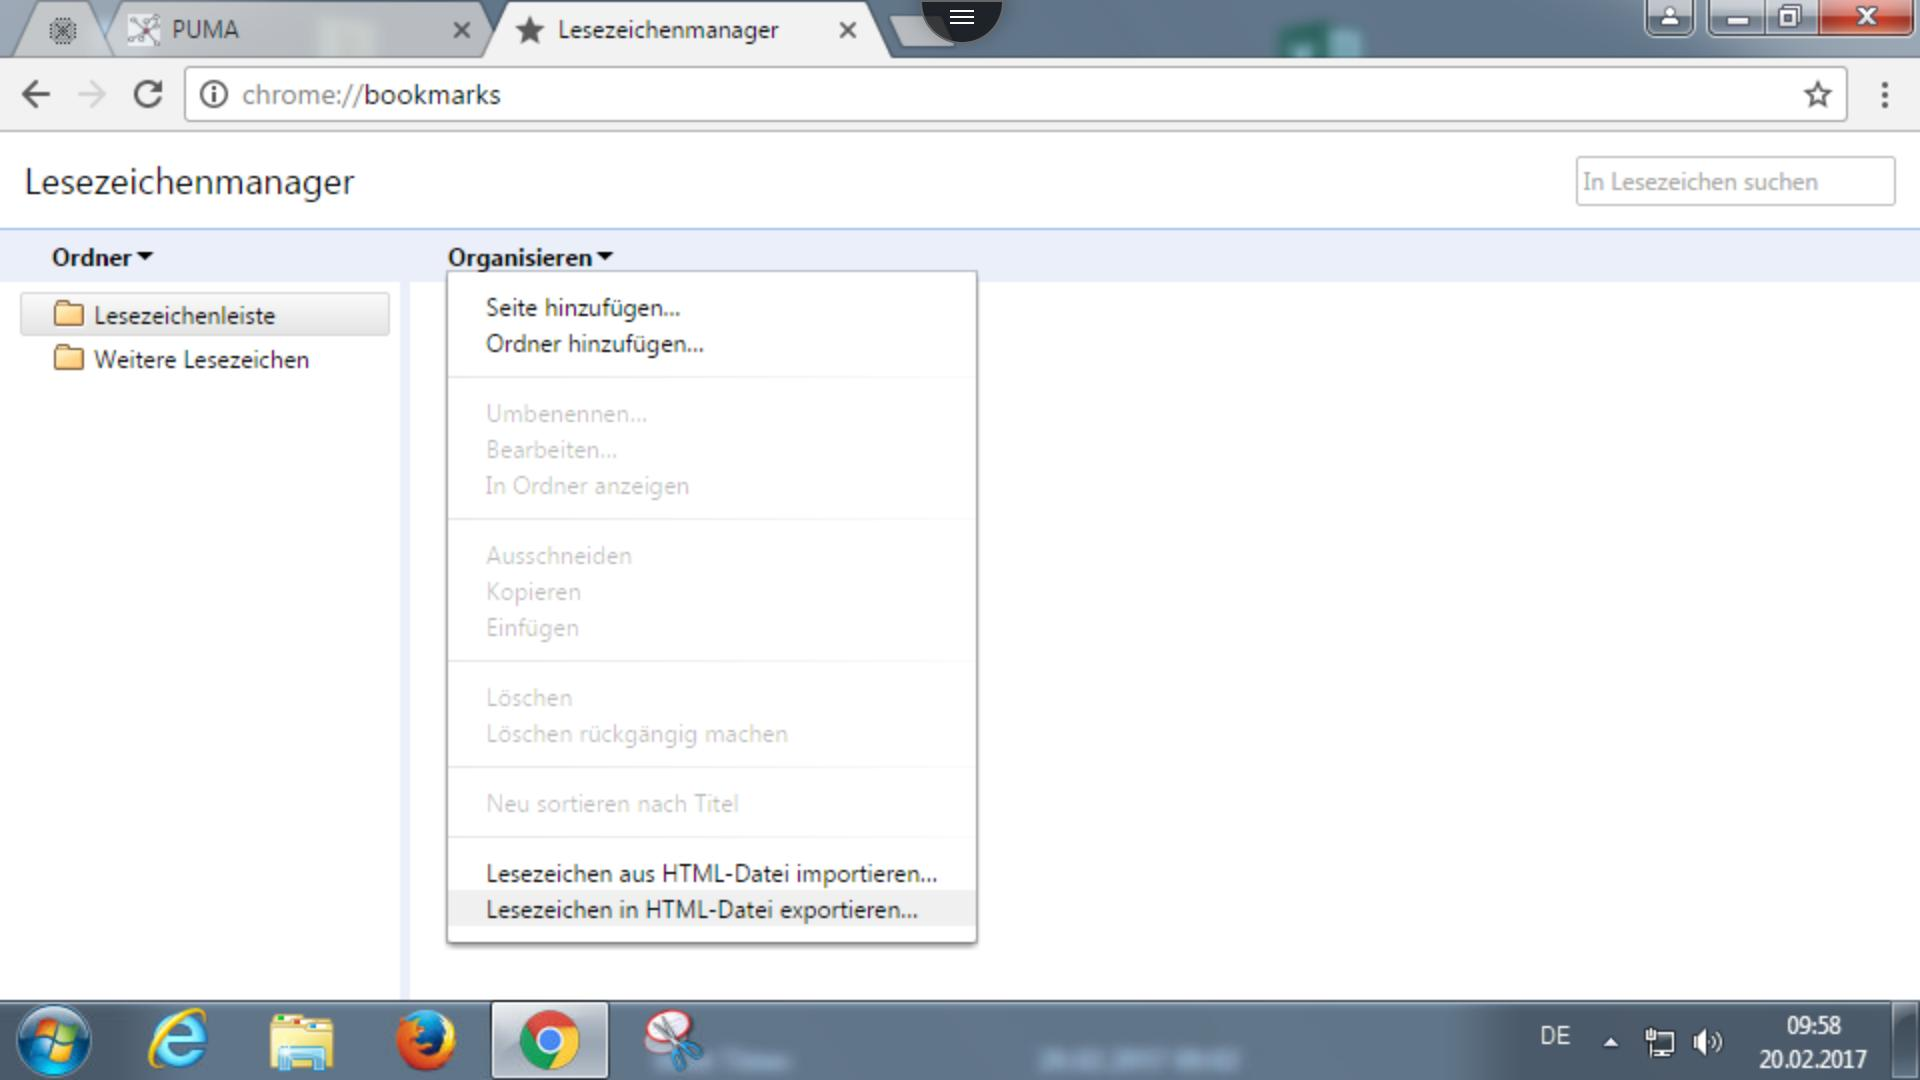
\includegraphics[width=9cm]{Bilder/Kapitel5/Lesezeichen_HTML_Chrome}}
 \caption{Lesezeichen in HTML-Datei exportieren}
 \label{fig:lesezeichenHtmlExportieren}
\end{figure}

\textbf{Firefox}
\newline Lesezeichen in Firefox\index{Firefox} können über das Lesezeichensymbol $\to$ \enquote{Lesezeichen verwalten} $\to$ \enquote{importieren und sichern} $\to$ \enquote{Lesezeichen nach HTML exportierem} rechts neben der Suchleiste als HTML-Datei zu exportieren werden.

\begin{figure}[h!]
 \centering
 \fbox{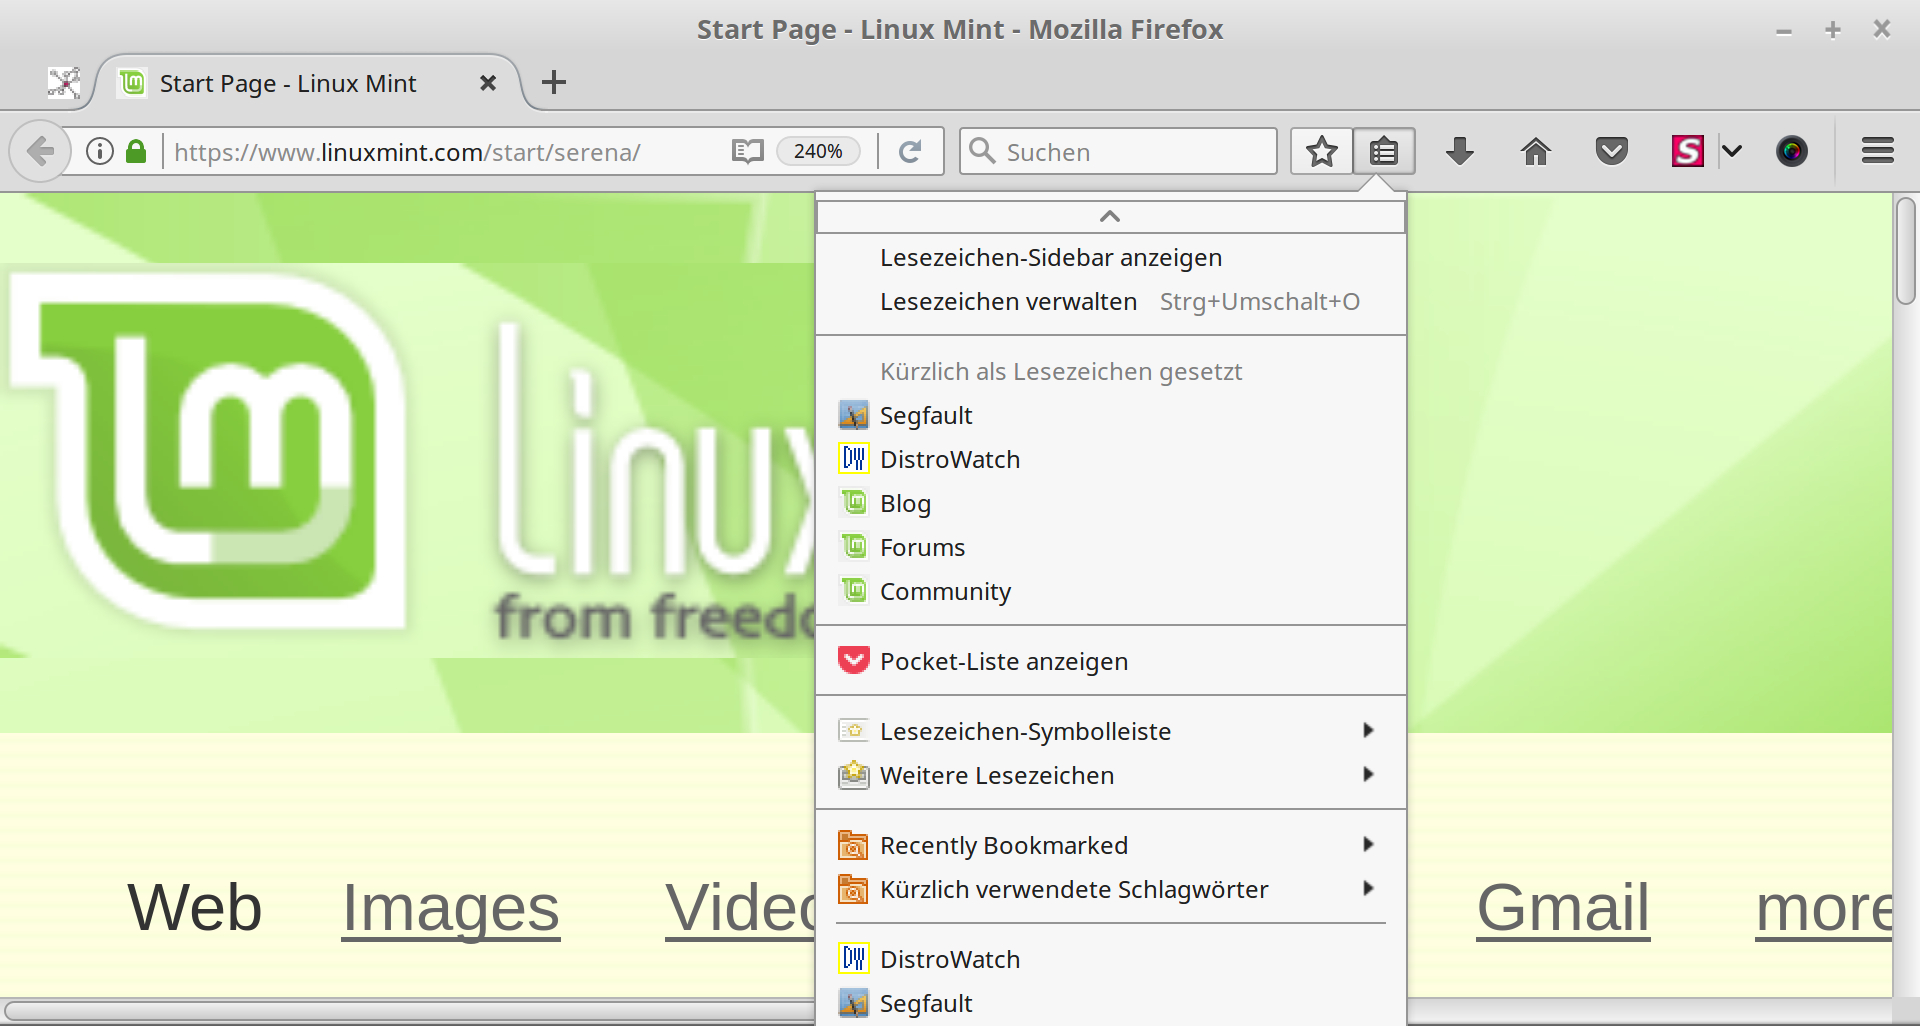
\includegraphics[width=11cm]{Bilder/Kapitel5/Firefox_Lesezeichen_verwalten}}
 \caption{Lesezeichen verwalten}
 \label{fig:lesezeichenVerwalten}
\end{figure}
 
\section{Browser-Add-ons\index{Add-ons}\label{sec:addon} und Bookmarklets}\label{sec:button}
PUMA bietet für Firefox Add-ons für PUMA-Schaltflächen an: \enquote{Mein PUMA}, \enquote{Publikation speichern} oder \enquote{Lesezeichen speichern}. Da die Add-ons mit jeder Firefox-Erweiterung angepasst werden müssen, können diese auch über \todo{woher?} manuell installiert werden. Beim installieren der Add-ons kann über \enquote{Instanz wechseln} \enquote{UB Stuttgart} ausgewählt werden. Als Alternative bieten sich die Bookmarklets an.\newline
%\begin{enumerate}
%\item Klicken Sie rechts oben im Firefox-Browser auf das Menü.
%\begin{figure}[h!]
 %\centering
 %\fbox{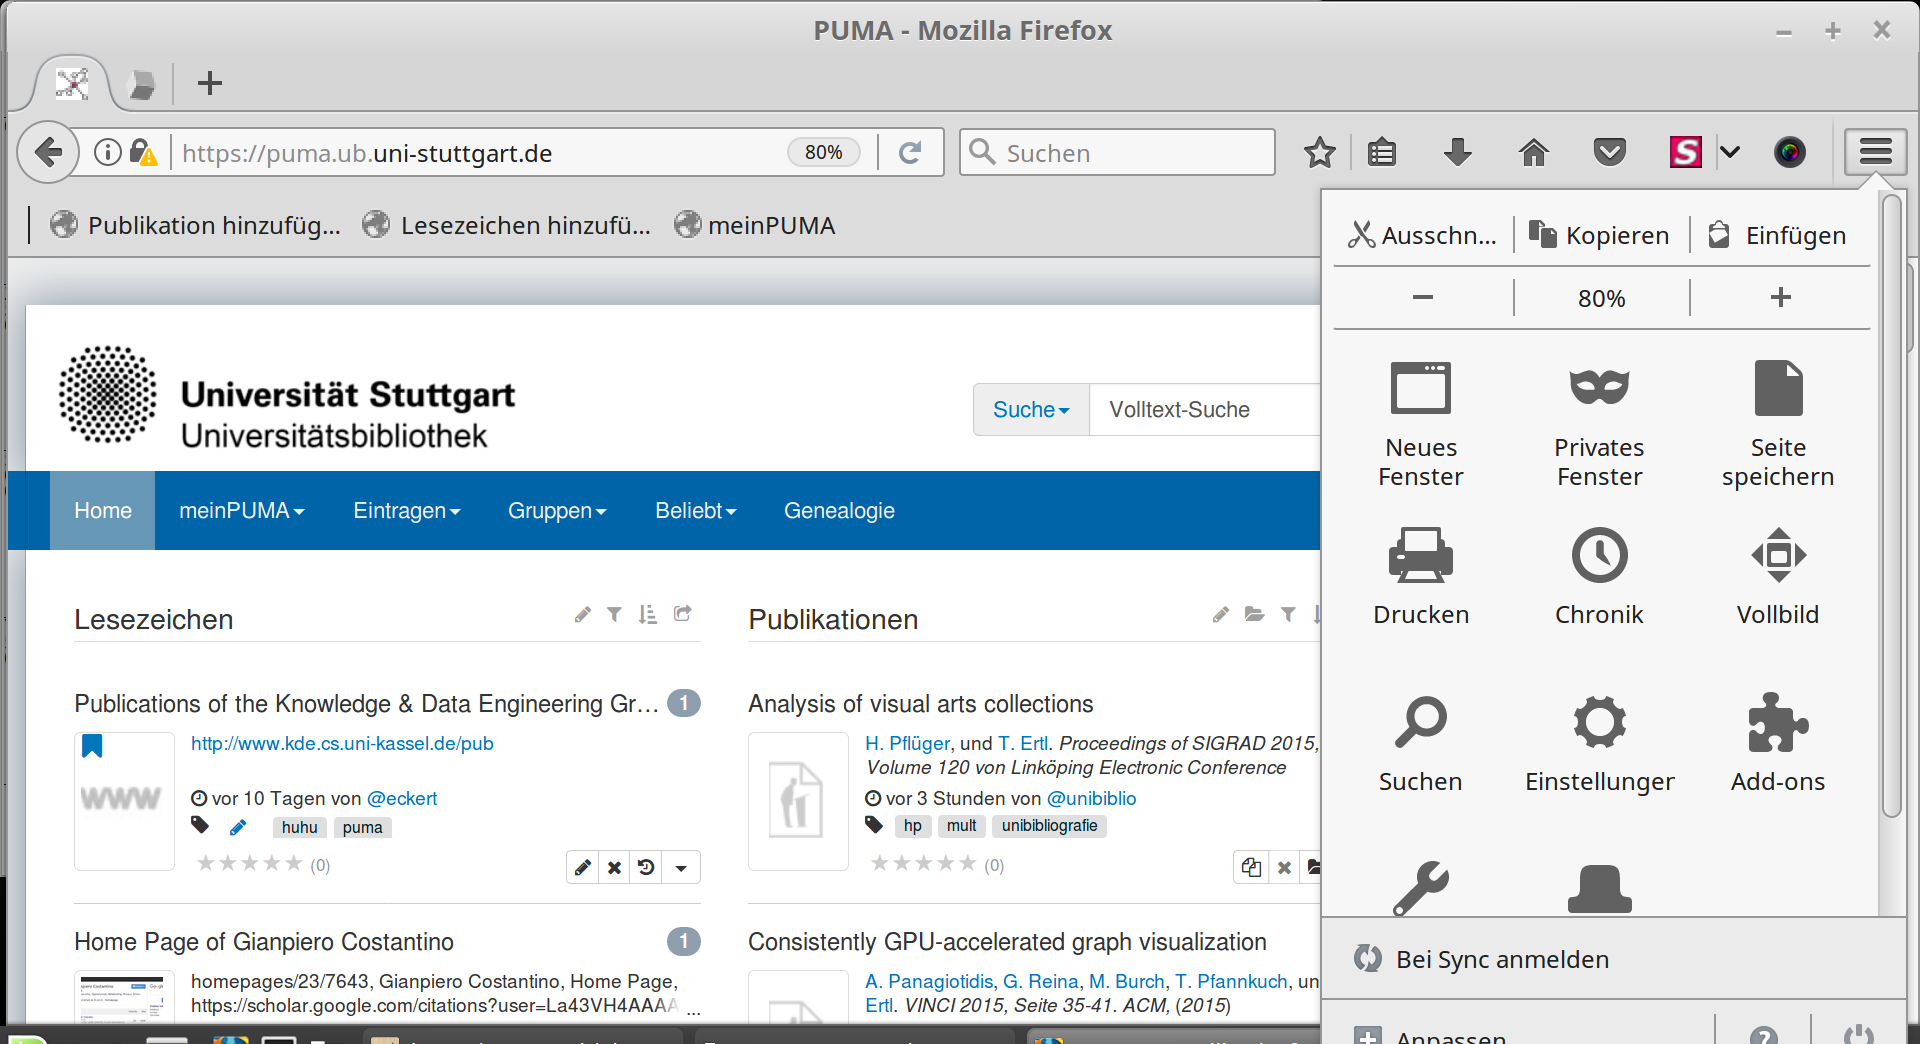
\includegraphics[width=11cm]{Bilder/Kapitel5/Menue_Firefox}}
 %\caption{Firefox-Browser}
 %\label{fig:firefoxBrowser}
%\end{figure} 
%\item Es öffnet sich das Menü, wählen Sie den Reiter \enquote{Add-ons} aus. 
%\item Geben Sie in die Suchleiste oben rechts \enquote{puma} ein.
%\item Es erscheint das Add-on \enquote{PUMA Buttons}. Installieren Sie die Buttons (Version 1.6.2).
\begin{figure}[h!]
 \centering
 \fbox{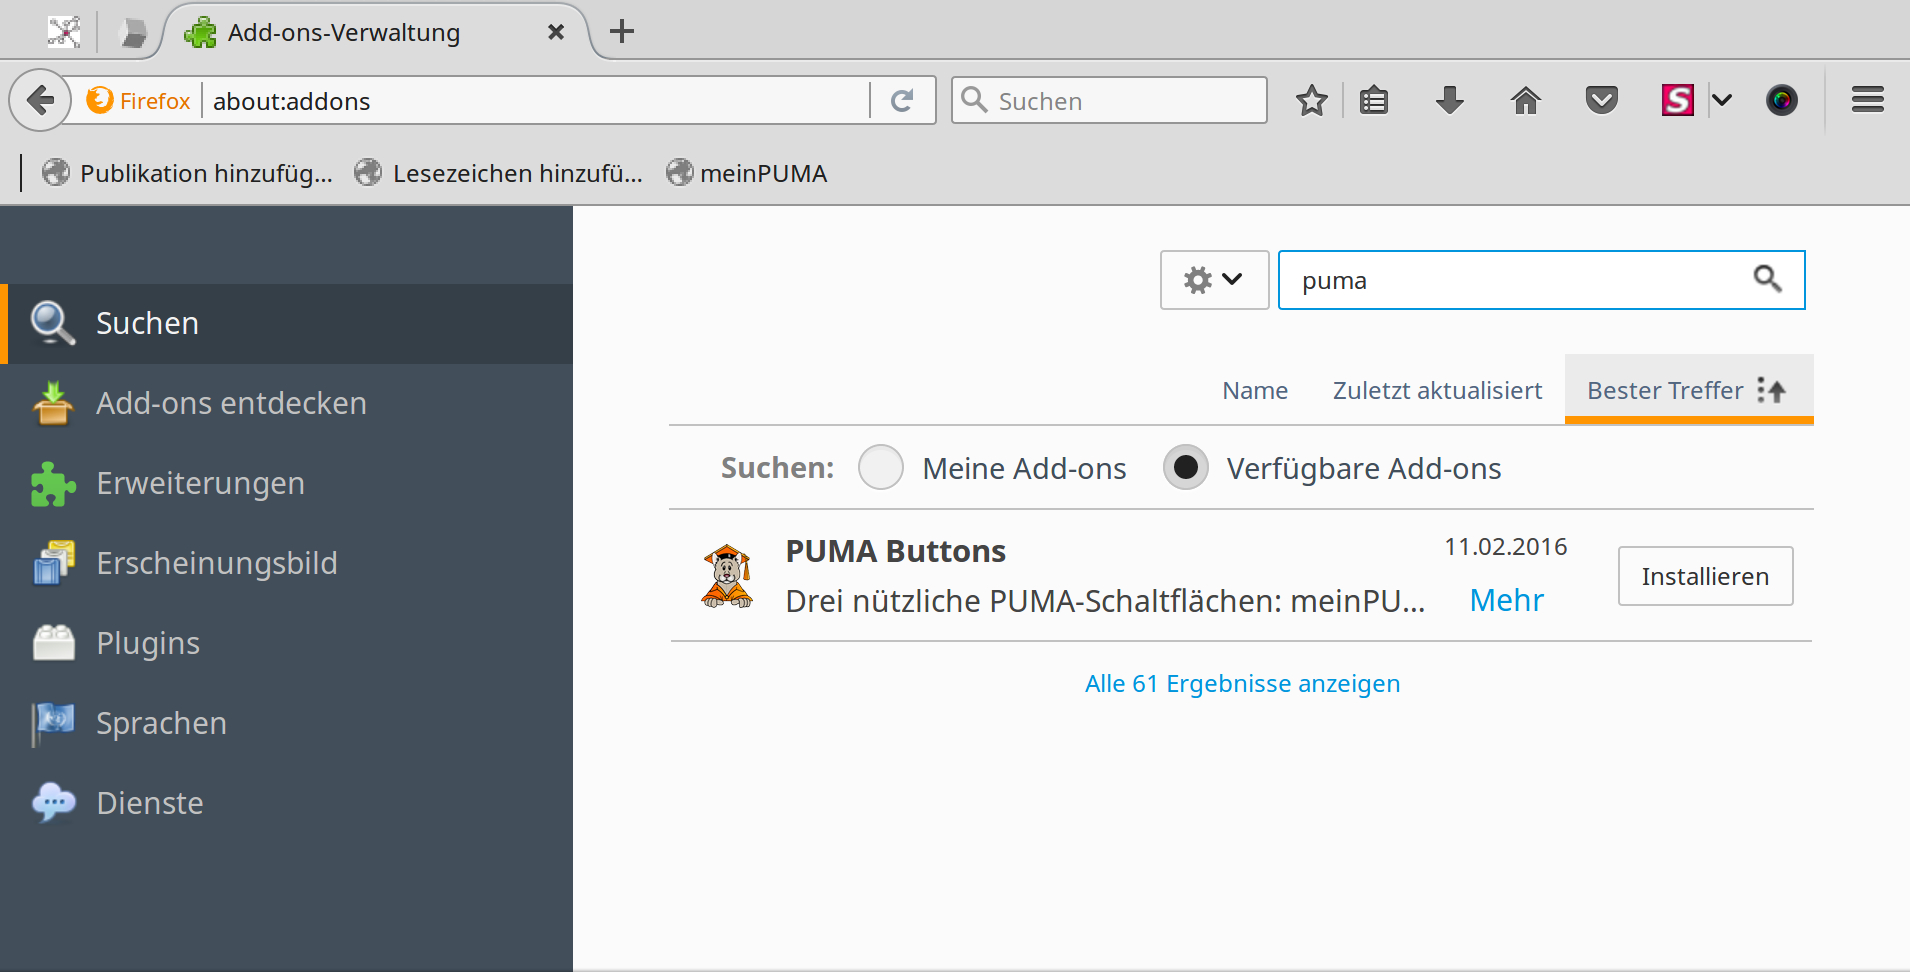
\includegraphics[width=11cm]{Bilder/Kapitel5/PUMA_Buttons}}
 \caption{Puma Buttons}
 \label{fig:pumaButtons}
\end{figure} 
%\item Klicken Sie anschließend auf \enquote{mehr} und scrollen auf der Seite runter bis zum Abschnitt \enquote{Instanz wechseln}. 
%\item Durch das Klicken auf \enquote{Instanz wechseln} öffnet sich eine Übersicht über alle verfügbaren PUMAs. Wählen Sie  \enquote{UB Stuttgart} aus und speichern Ihre Wahl.
%\item Falls die Buttons nicht sofort in der Taskleiste neben dem Menüsymbol  erscheinen, schließen Sie Firefox. Beim erneuten Öffnen des Firefox-Browsers wurden die Buttons eingerichtet.
%\end{enumerate}
Die Bookmarklet-Buttons\index{Bookmarklet-Buttons} ermöglichen ein schnelles Arbeiten mit PUMA, während der Recherche im Internet. Es vereinfacht das Eintragen von Publikationen und Lesezeichen. Mit dem PUMA-Home Bookmarklet-Button gelangt man direkt zu PUMA. Dafür die Buttons\footnote{\url{https://puma.ub.uni-stuttgart.de/buttons}} einfach in die Lesezeichen-Leiste ziehen.
\begin{figure}[h!]
 \centering
 \fbox{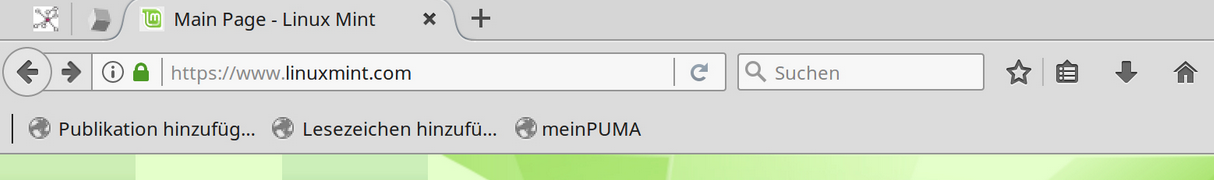
\includegraphics[width=11cm]{Bilder/Kapitel5/Bookmarklet-Buttons}}
 \caption{Bookmarklet-Buttons}
 \label{fig:bookmarkletButtons}
\end{figure} 

\section{Ablage}
\label{sec:ablage}
Die Ablage\index{Ablage} ermöglicht es eigene und fremde Publikationen zusammenzustellen und Aktionen für diese gesammelt durchzuführen (Stapelverarbeitung). So können zum Beispiel Literaturlisten für den Export zusammengestellt werden oder alle ausgewählten Publikationen mit dem gleichen \tag versehen werden. Dazu auf das Ordnersymbol \enquote{Diese Publikation zur Ablage hinzufügen} klicken. Die Publikationen gelangen direkt in die Ablage, die über das Personensymbol geöffnet werden kann. Am Personensymbol wird auch die Anzahl der abgelegten Publikationen angezeigt. \todo[inline]]{Eingang? Hinweis und link}
Über das (graue) Stiftsymbol oberhalb der gesammelten Einträge können alle Einträge in der Ablage bearbeitet werden. Folgende Aktionen stehen zur Verfügung:
\begin{itemize}
\item BibTex-Schlüssel normalisieren
\item Sichtbarkeit ändern
\item Einträge löschen
\item \tags an alle Einträge hinzufügen
\item \tags einzelner Einträge bearbeiten
\end{itemize}
\begin{figure}[h!]
 \centering
 \fbox{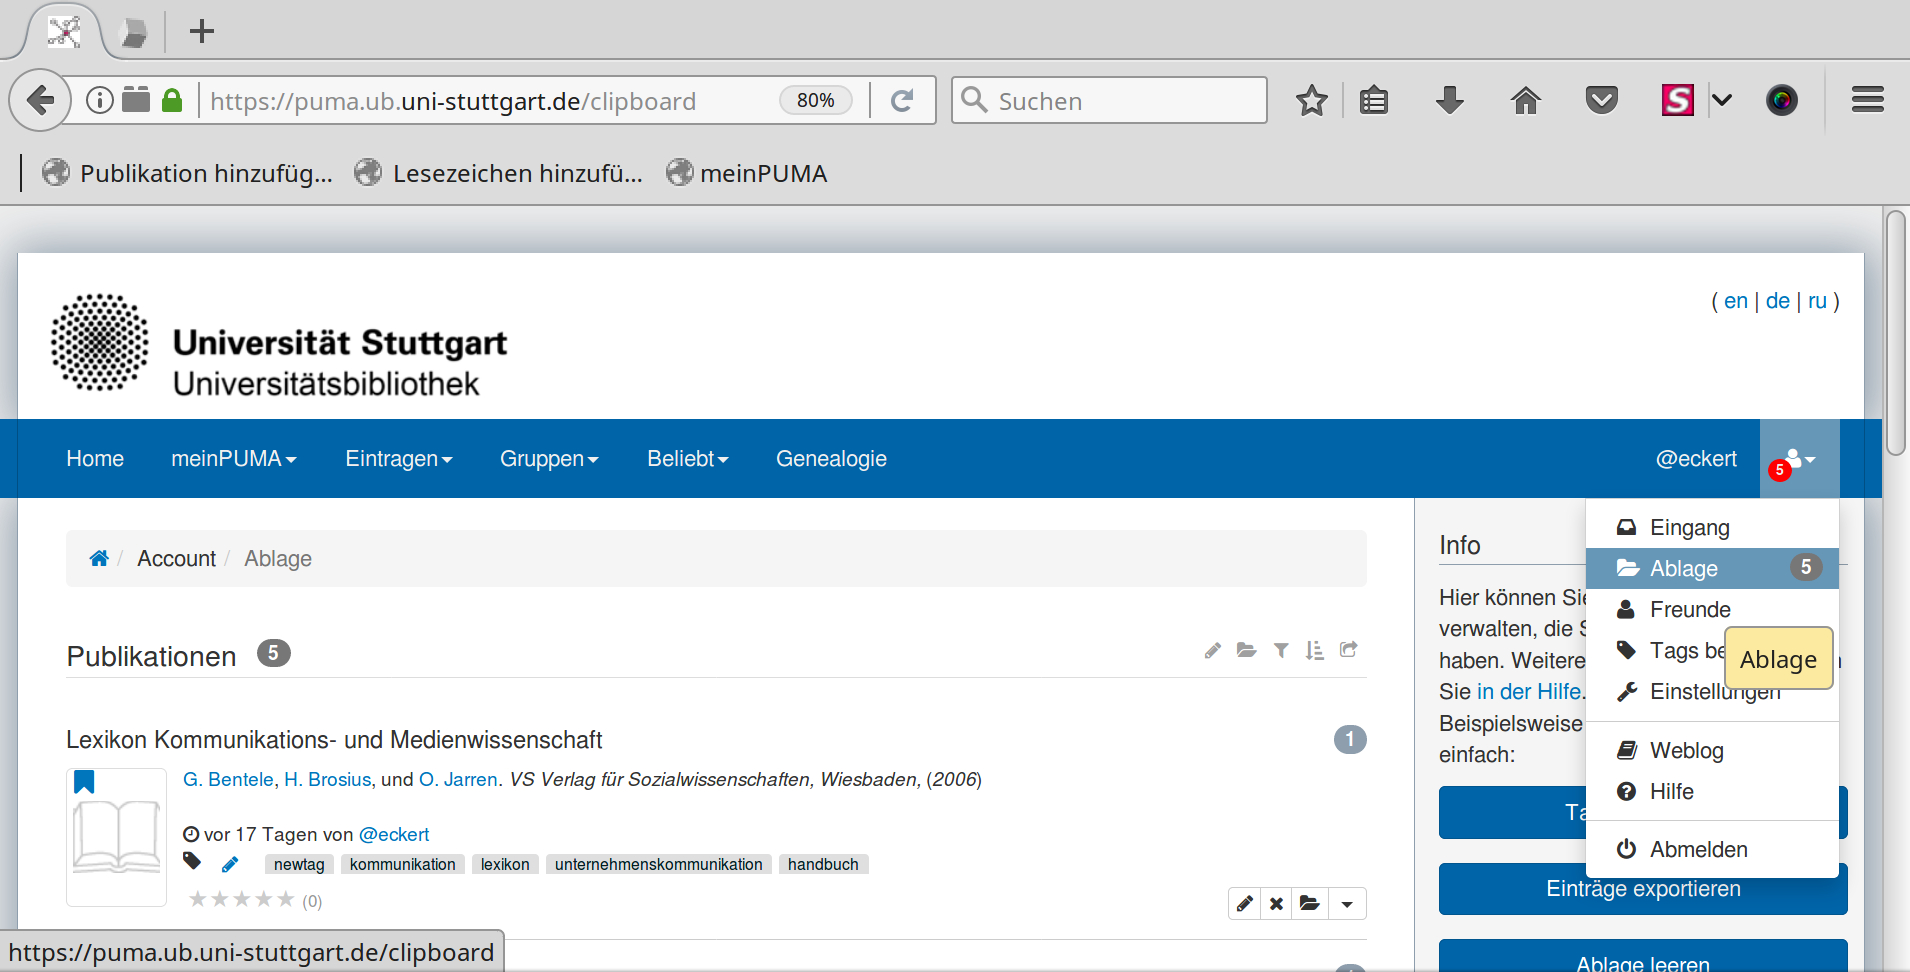
\includegraphics[width=11cm]{Bilder/Kapitel5/Ablage}}
 \caption{Die Ablage}
 \label{fig:ablage}
\end{figure} 
Über das (graue) Ordnersymbol neben dem Stiftsymbol kann die gesamte Ablage geleert werden. Um einzelne Einträge zu entfernen, das Ordnersymbol neben dem Eintrag klicken. 
\begin{tip}Über das schwarze \enquote{X} (diese Publikation aus Ihrer Sammlung löschen)) wird die Publiaktion auch in der eigenen Sammlung gelöscht und kann nicht wiederhergestellt werden.
\end{tip}
Teilweise können die beschriebenen Funktionen können auch über die rechte Menüleiste ausgewählt werden.
%\end{wrapfigure}
%\section{Frischalten erweiterter Funktionen}
%\label{sec:freischaltenErweiterterFunktionen}
%Bei PUMA gibt es die Unterscheidung zwischen einfachen\index{Funktionen!Einfache} und erweiterten Funktionen\index{Funktionen!Erweiterte}. In den Grundeinstellungen stehen jedem Nutzer, bei dessen Anmeldung bei PUMA, die einfachen Funktionen zur Verfügung. Durch das Freischalten der erweiterten Funktionen kommen weitere Funktionen hinzu, sodass Sie mehr Möglichkeiten haben, PUMA zu nutzen.  Wenn Sie die erweiterten Funktionen freischalten möchten, gehen Sie wie folgt vor:
%\begin{enumerate}
    %\item Klicken Sie auf das Personensymbol. Ein Dropdown-Menü öffnet sich, klicken Sie auf \enquote{Einstellungen}.
    %\item Es öffnet sich die Einstellungs-Seite. Klicken Sie oben auf den Reiter \enquote{Einstellungen}.
    %\item Unter dem Bereich \enquote{Layouts Ihrer Tagbox und Ihrer Eintragslisten} befindet sich das Feld \enquote{Erscheinungsbild}. Sie können nun zwischen den Standardeinstellungen \textit{Erweitert} (Alle Optionen werden stets angezeigt) oder \textit{Einfach} (Einige \enquote{Experten}-Optionen werden standardmäßig nicht angezeigt) wählen.

\section{Konto auflösen}
\label{sec:kontoAufloesen} 
\subsection{Konto löschen}\index{Konto!löschen} \label{subsec:kontoAufloesen}
\subsection{Ausscheiden aus der Uni}\index{Konto!auflösen} \label{subsec:kontoLoeschen}
\todo[inline]{braucht es dazu einen eigenen Abschnitt, oben kurz beschrieben}
